\chapter{Tokyo}
\section*{28 juillet 2015}
Je suis resté un peu plus d'une semaine à Tokyo pour visiter et faire la demande de visa pour la Chine. \newline
 4 déplacements à l'ambassade de Chine et un peu de galère mais j'ai obtenu le visa pour 1 mois. \newline
 Les premiers jours j'ai été hébergé par Akira, dans son tout petit appartement. \newline
 \newline
\centerline{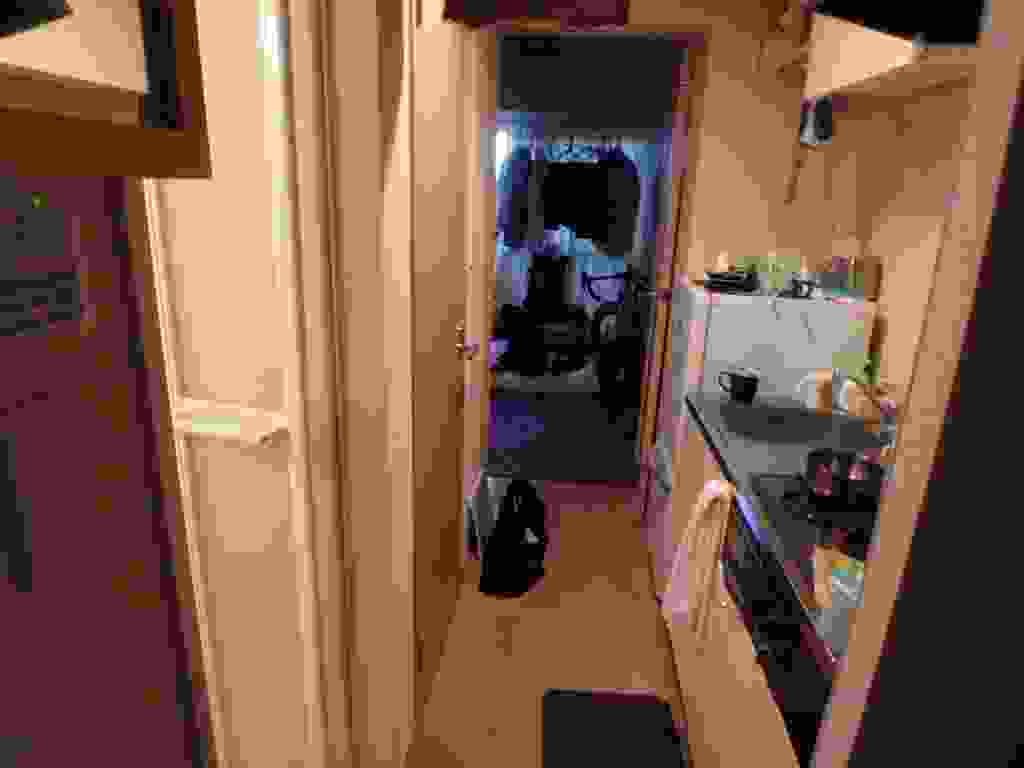
\includegraphics[width=\mywidth]{../wp-content/uploads/2015/07/P7195495-1024x768.jpg} } 
 \newline
 Il a beaucoup voyagé en vélo, en Europe, en Afrique et en Amérique. Maintenant il travaille à Tokyo, de gros horaires, je n'ai pas passé beaucoup de temps avec lui ! \newline
 \newline
\centerline{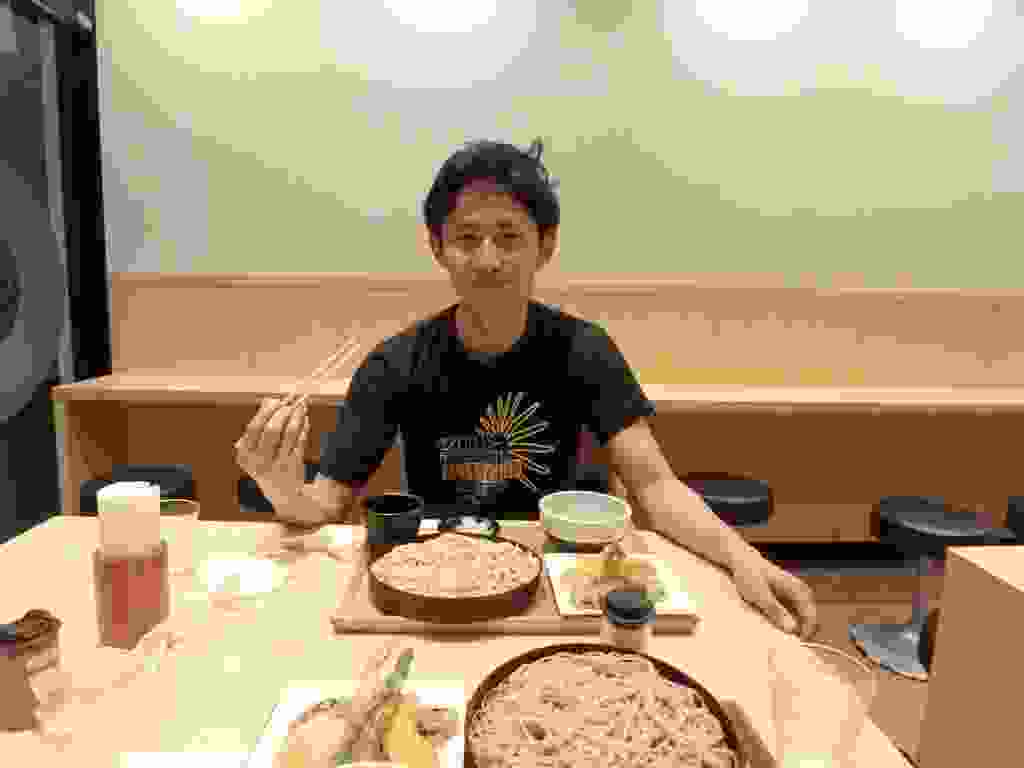
\includegraphics[width=\mywidth]{../wp-content/uploads/2015/07/P7170025-1024x768.jpg} } 
 \newline
 Tokyo est une ville immense avec au moins une dizaine de quartiers intéressants à visiter, chacun avec son ambiance et ses particularités. \newline
 J'ai commencé par Shinjuku où j'ai acheté un nouvel appareil photo dans un des multiples magasins d'objets électroniques. En plus les magasins au Japon sont tax free pour les étrangers. \newline
 \newline
\centerline{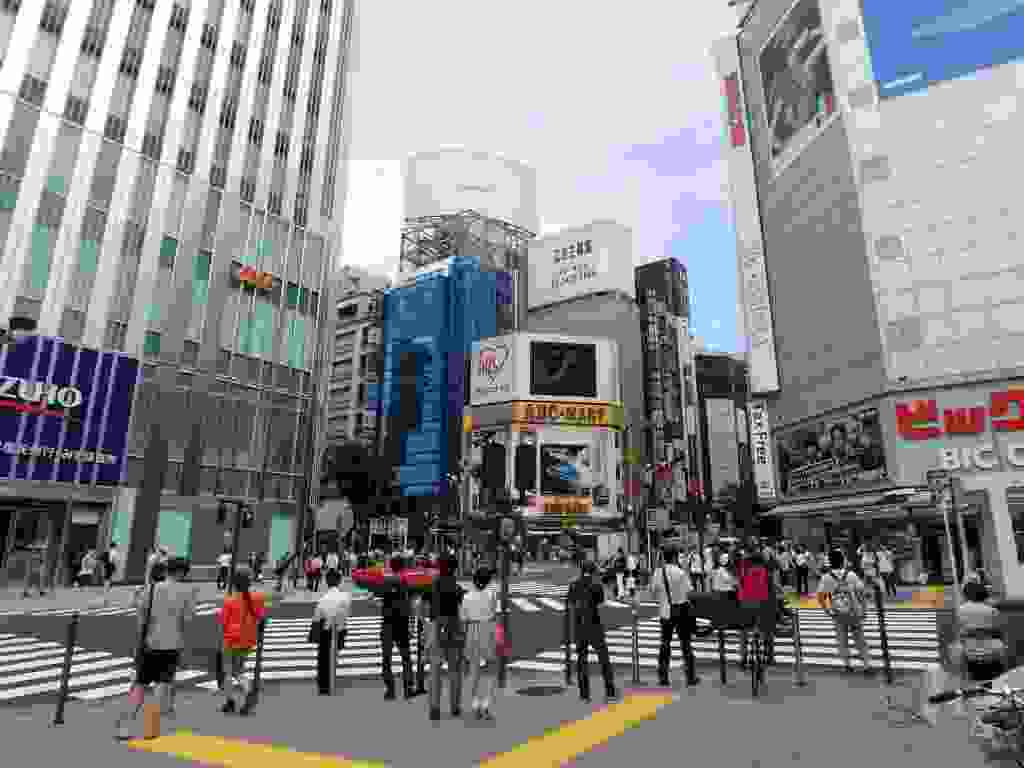
\includegraphics[width=\mywidth]{../wp-content/uploads/2015/07/OI000006-1024x768.jpg} } 
 \newline
 Vue en haut de l'immeuble du Tokyo Metropolitan Government \newline
 \newline
\centerline{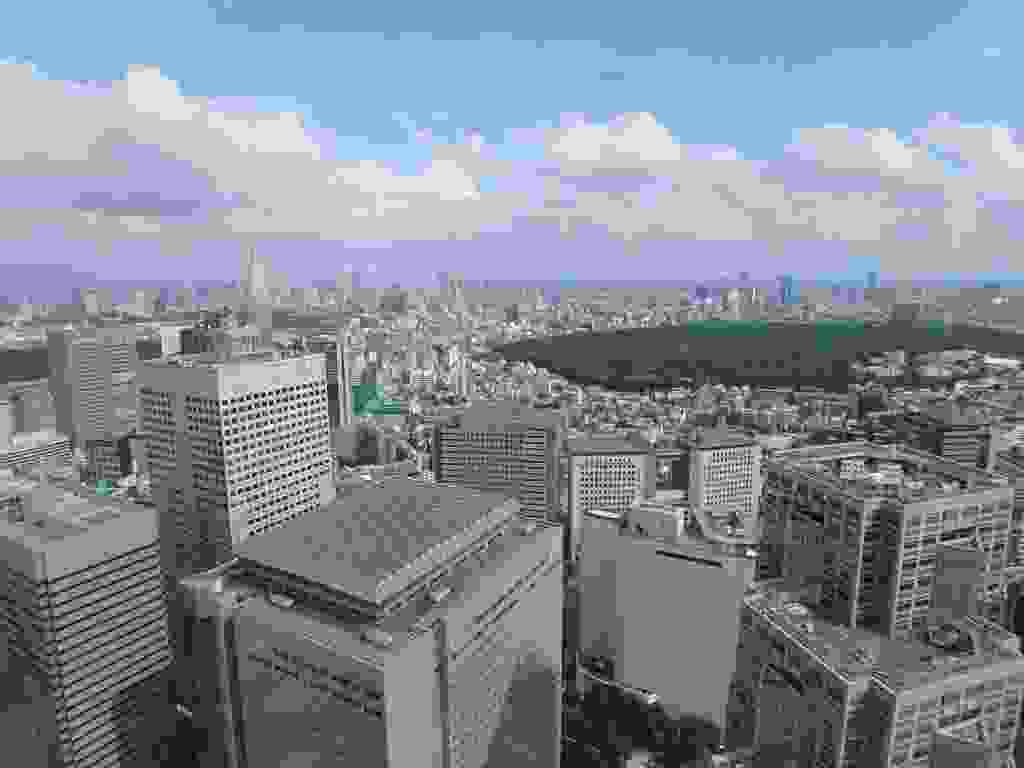
\includegraphics[width=\mywidth]{../wp-content/uploads/2015/07/OI000010-1024x768.jpg} } 
 \newline
 Balade dans le parc Shinjuku Gyoen \newline
 \newline
\centerline{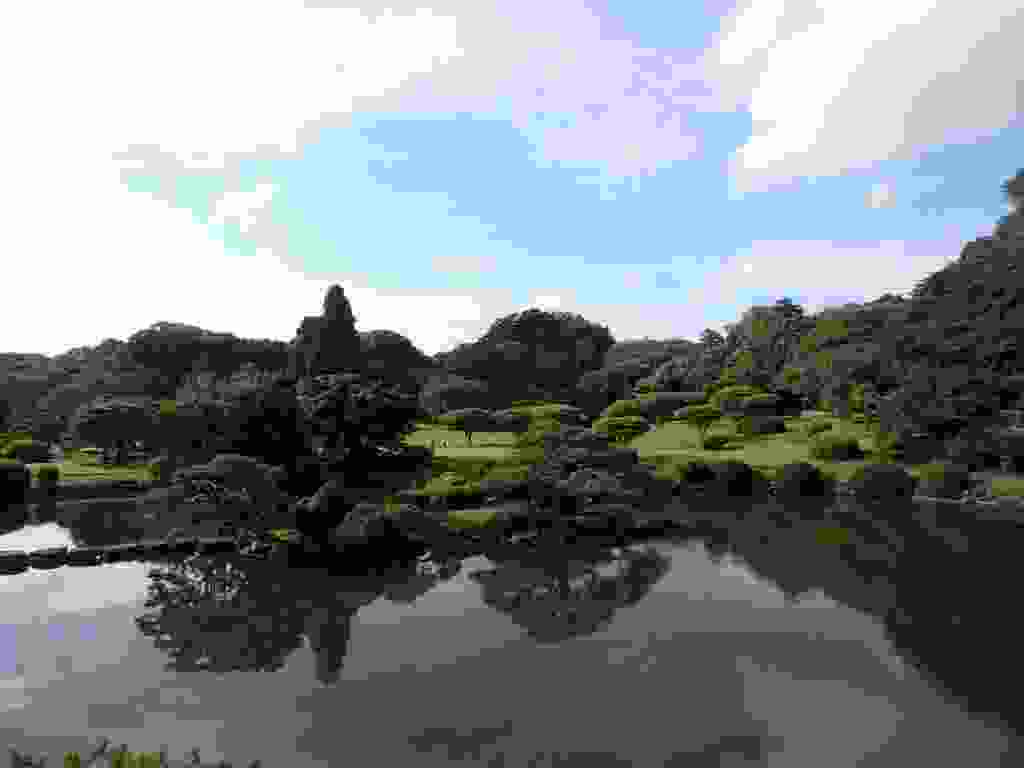
\includegraphics[width=\mywidth]{../wp-content/uploads/2015/07/OI000020-1024x768.jpg} } 
 \newline
 \newline
\centerline{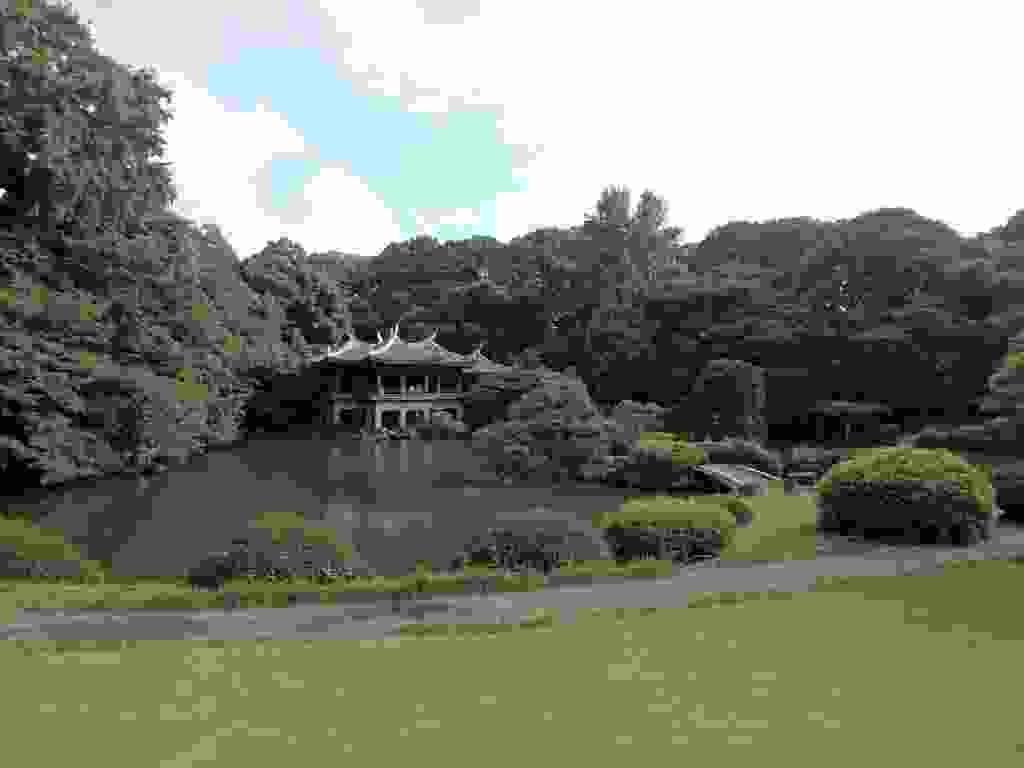
\includegraphics[width=\mywidth]{../wp-content/uploads/2015/07/OI000013-1024x768.jpg} } 
 \newline
 Le petit quartier de Golden Gai Shinjuku : des centaines de minuscules bars regroupés dans 5 ou 6 ruelles. \newline
 \newline
\centerline{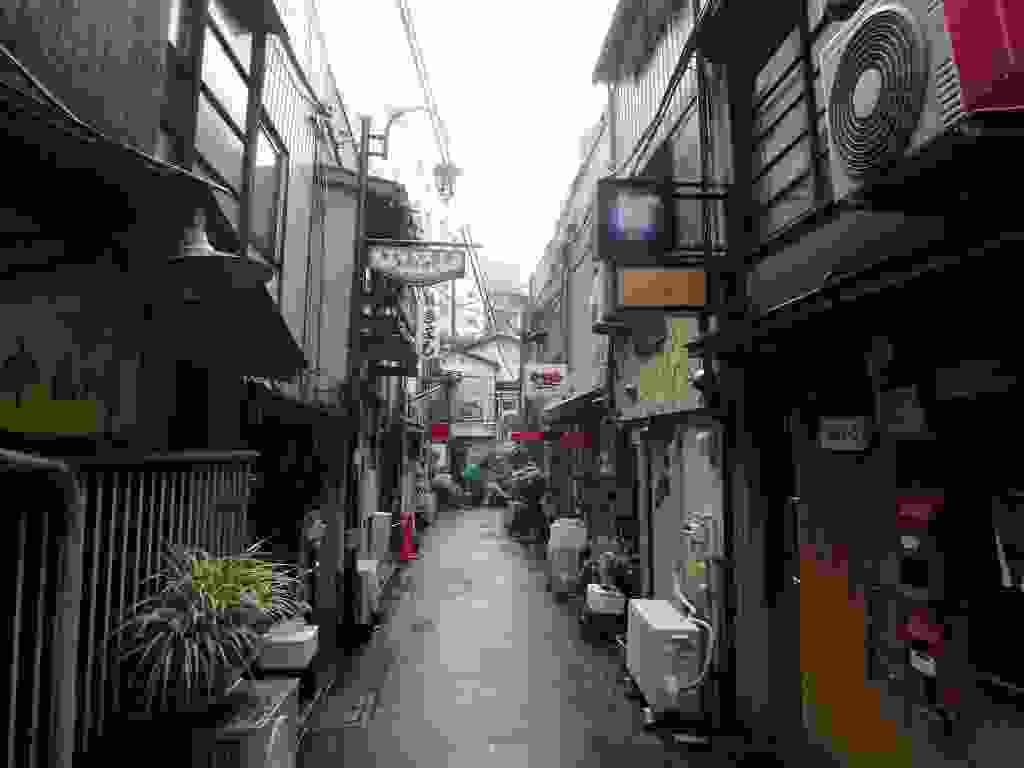
\includegraphics[width=\mywidth]{../wp-content/uploads/2015/07/P7245595-1024x768.jpg} } 
 \newline
 Marunouchi : le quartier central avec le palais impérial et son parc. \newline
 \newline
\centerline{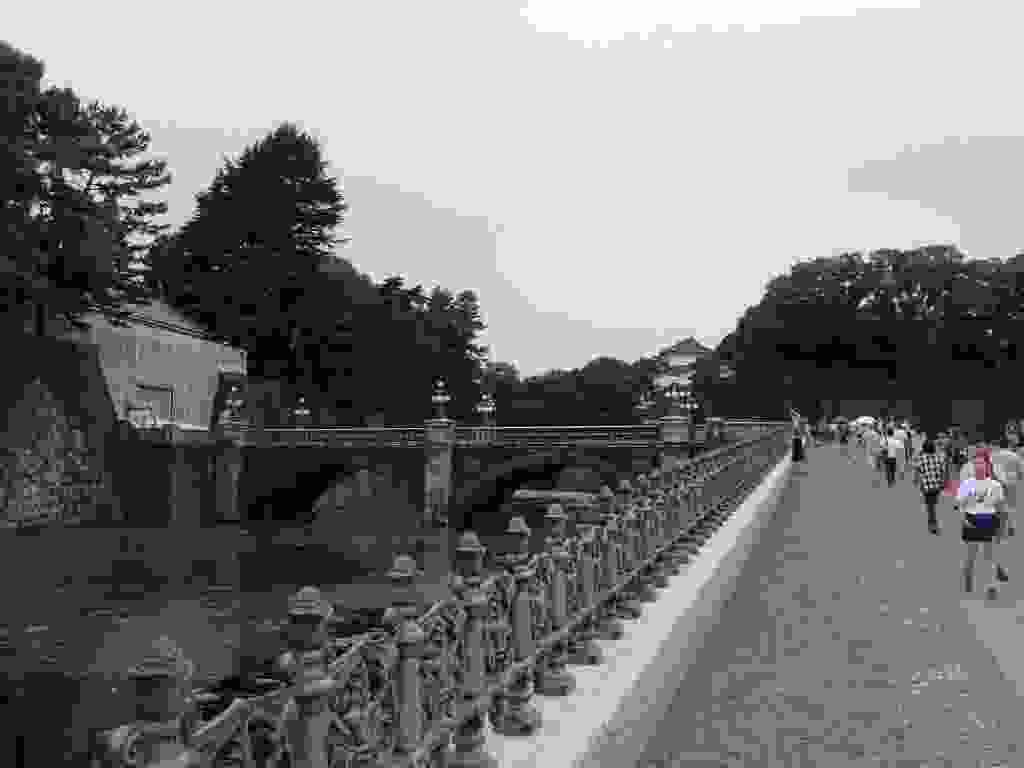
\includegraphics[width=\mywidth]{../wp-content/uploads/2015/07/P7185407-1024x768.jpg} } 
 \newline
 \newline
\centerline{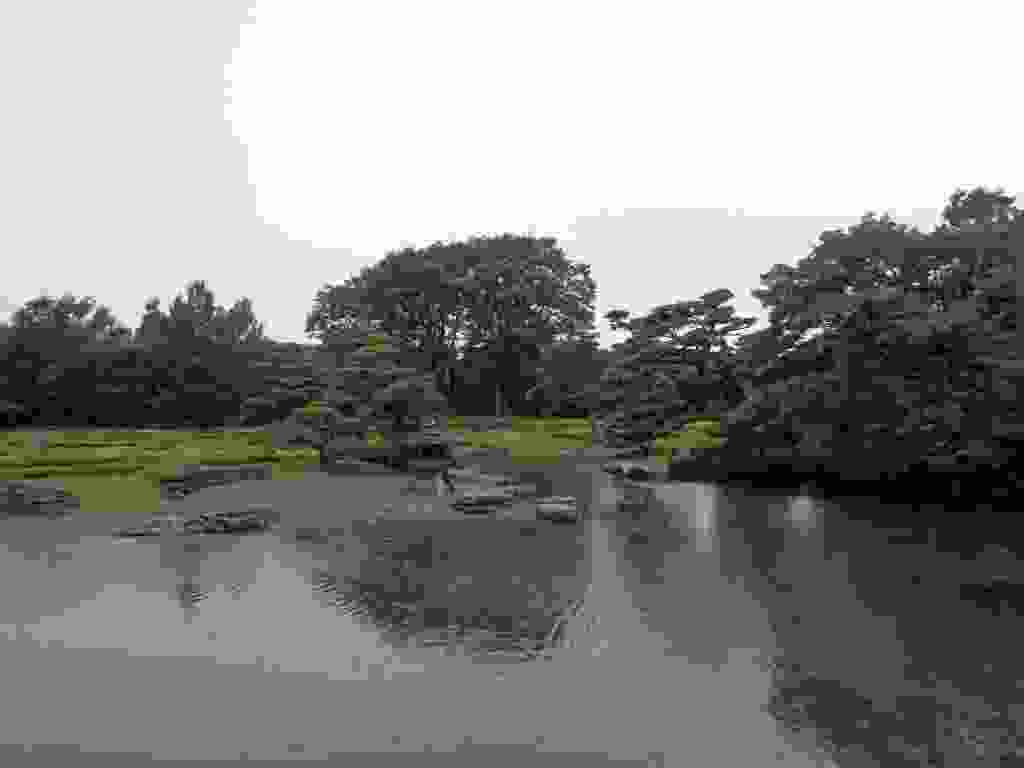
\includegraphics[width=\mywidth]{../wp-content/uploads/2015/07/P7185419-1024x768.jpg} } 
 \newline
 \newline
\centerline{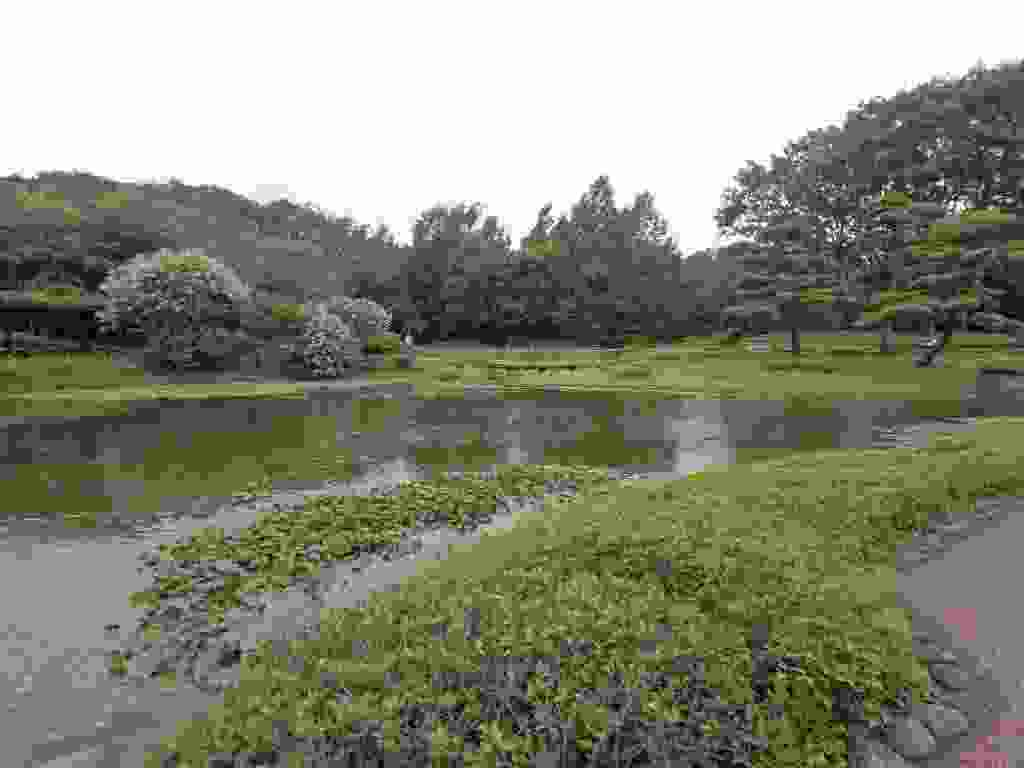
\includegraphics[width=\mywidth]{../wp-content/uploads/2015/07/P7185418-1024x768.jpg} } 
 \newline
 \newline
\centerline{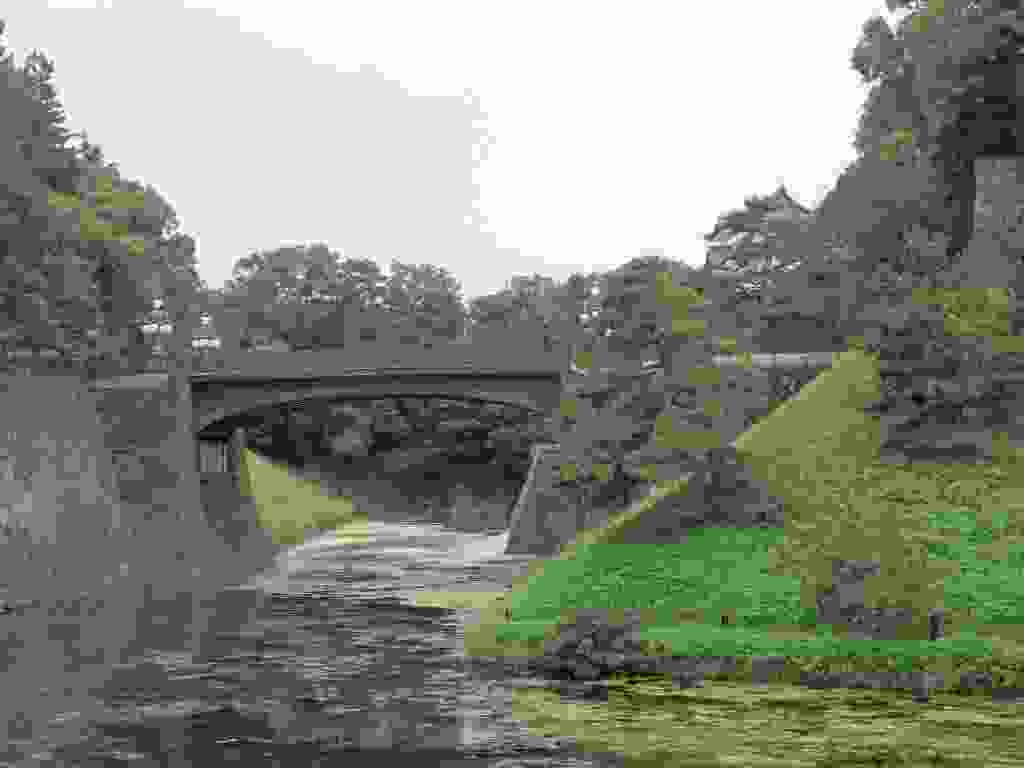
\includegraphics[width=\mywidth]{../wp-content/uploads/2015/07/P7185409-1024x768.jpg} } 
 \newline
 \newline
\centerline{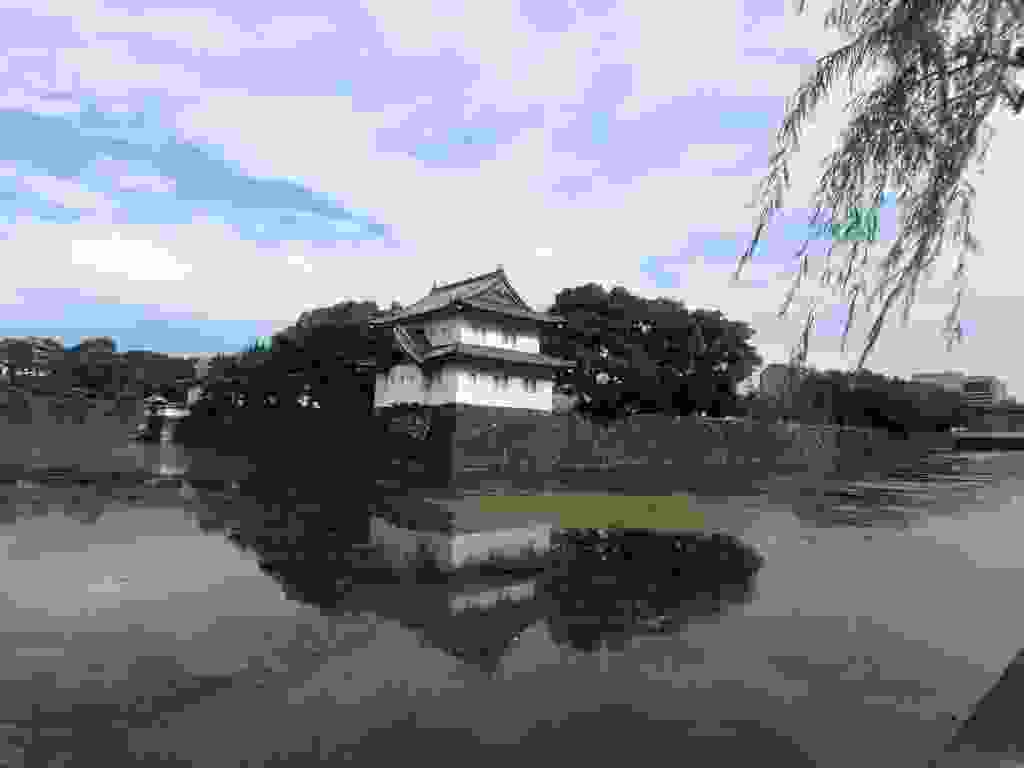
\includegraphics[width=\mywidth]{../wp-content/uploads/2015/07/P7185385-1024x768.jpg} } 
 \newline
 A côté le quartier Ginza et le marché de Tsukiji où on trouve de bons sushis. \newline
 \newline
\centerline{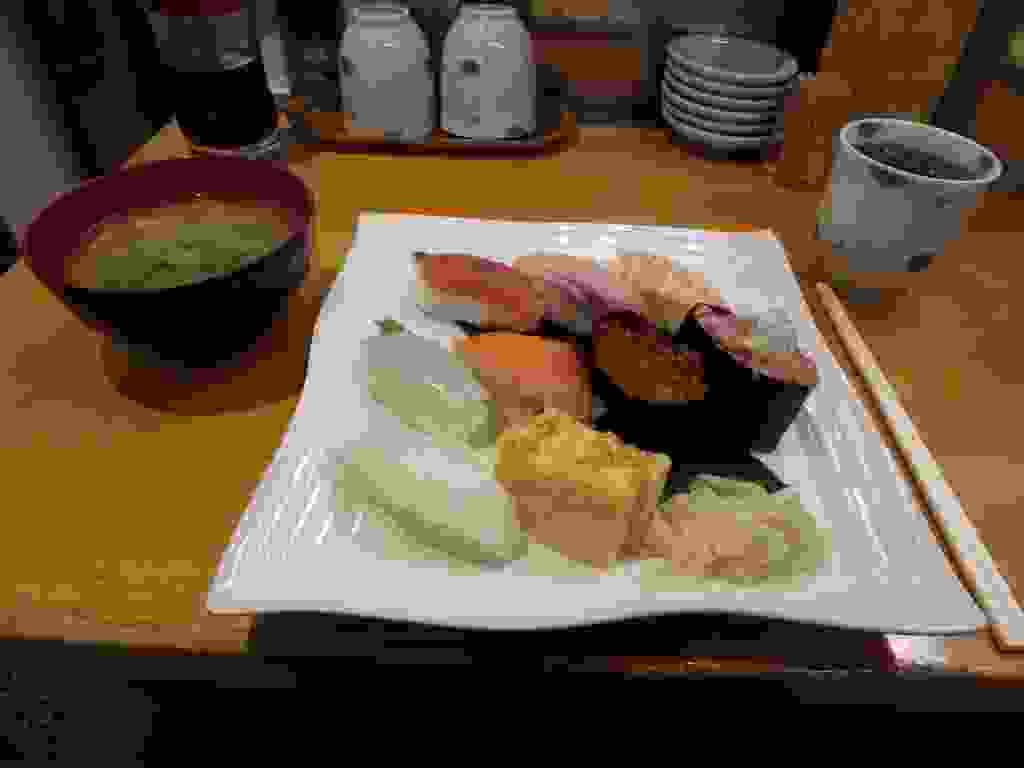
\includegraphics[width=\mywidth]{../wp-content/uploads/2015/07/P7185399-1024x768.jpg} } 
 \newline
 \newline
\centerline{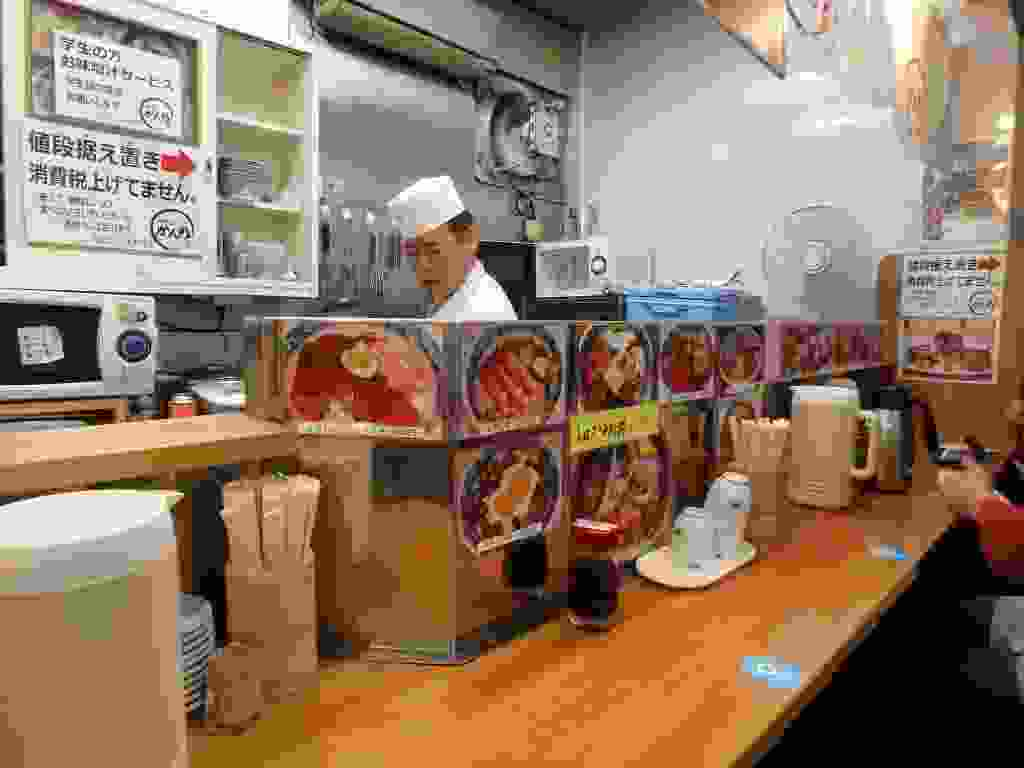
\includegraphics[width=\mywidth]{../wp-content/uploads/2015/07/P7185396-1024x768.jpg} } 
 \newline
 Pour acheter un couteau c'est la aussi \newline
 \newline
\centerline{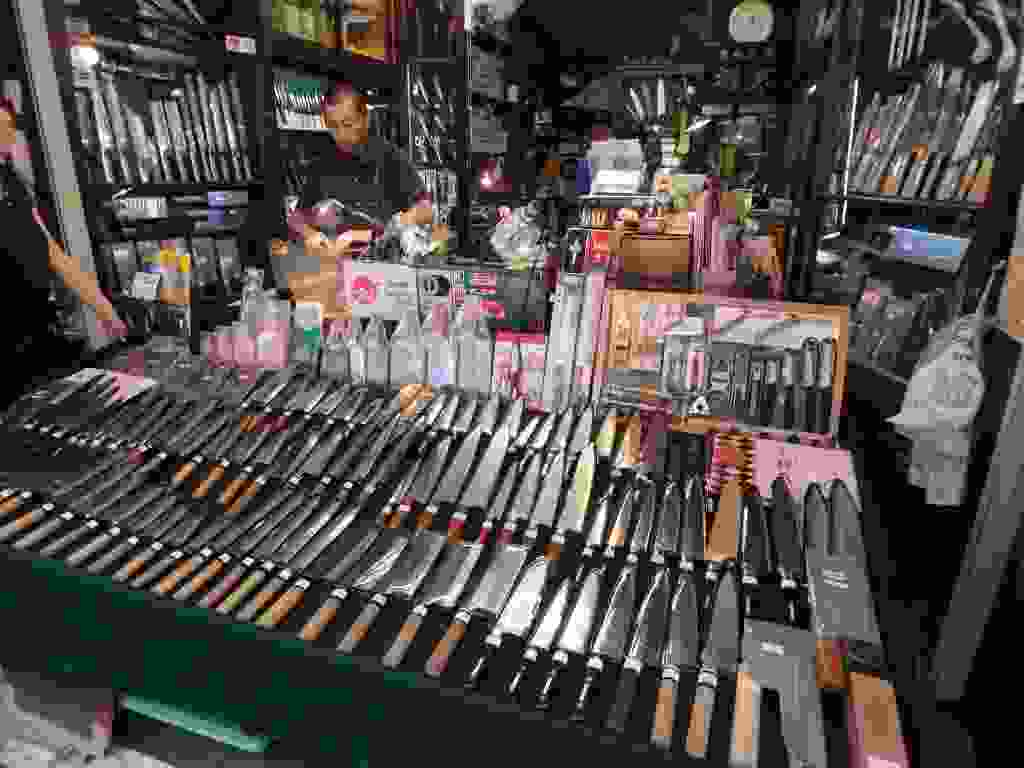
\includegraphics[width=\mywidth]{../wp-content/uploads/2015/07/P7185402-1024x768.jpg} } 
 \newline
 Shibuya : des centres commerciaux immenses et le fameux carrefour avec des passages piétons dans tous les sens. \newline
 \newline
\centerline{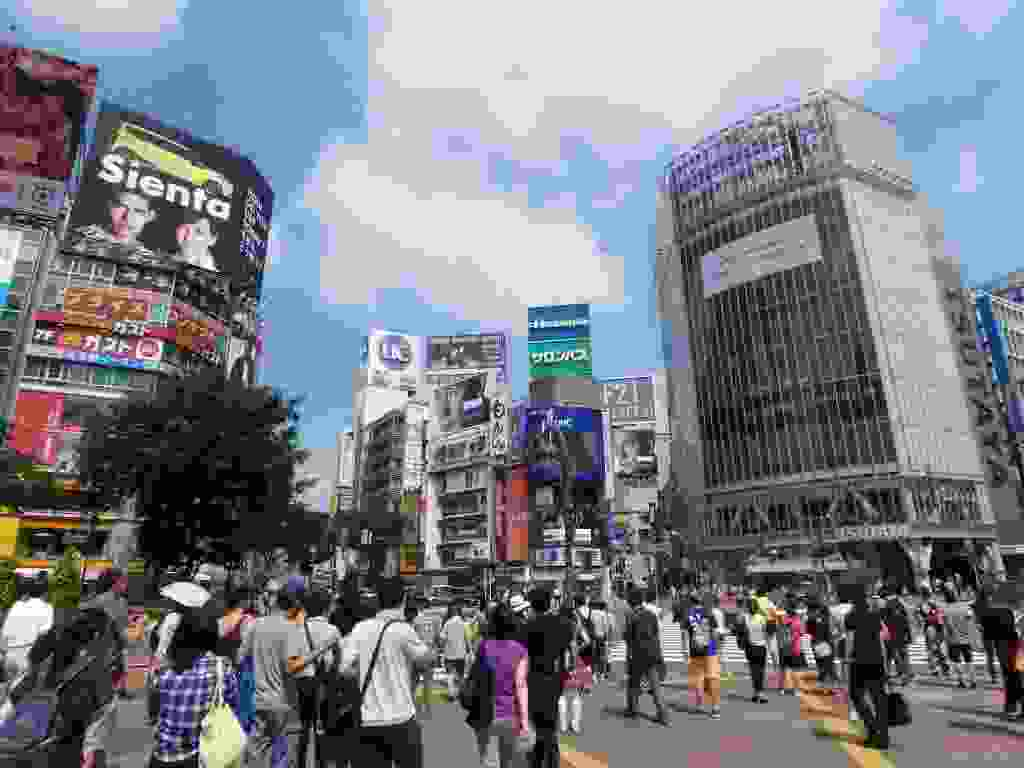
\includegraphics[width=\mywidth]{../wp-content/uploads/2015/07/P7205499-1024x768.jpg} } 
 \newline
 \newline
\centerline{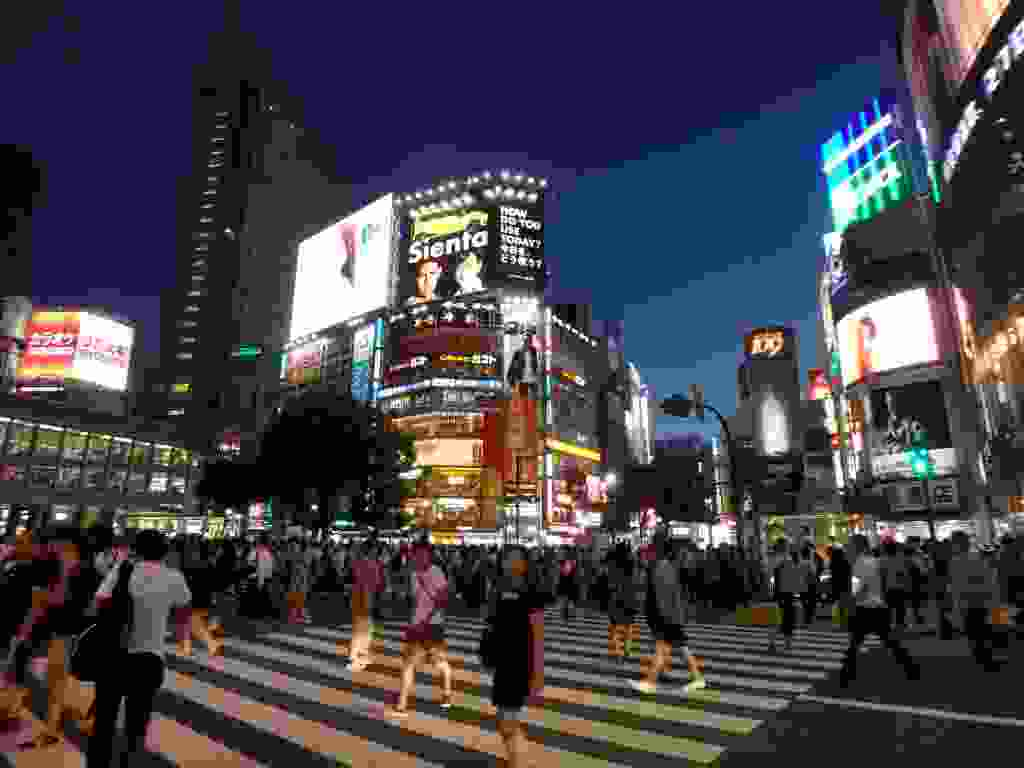
\includegraphics[width=\mywidth]{../wp-content/uploads/2015/07/P7225576-1024x768.jpg} } 
 \newline
 A côté le shrine Meiji Jingu. Au Japon, on trouve soit des temples bouddhistes soit des shrines qui appartiennent à la religion Shinto. \newline
 \newline
\centerline{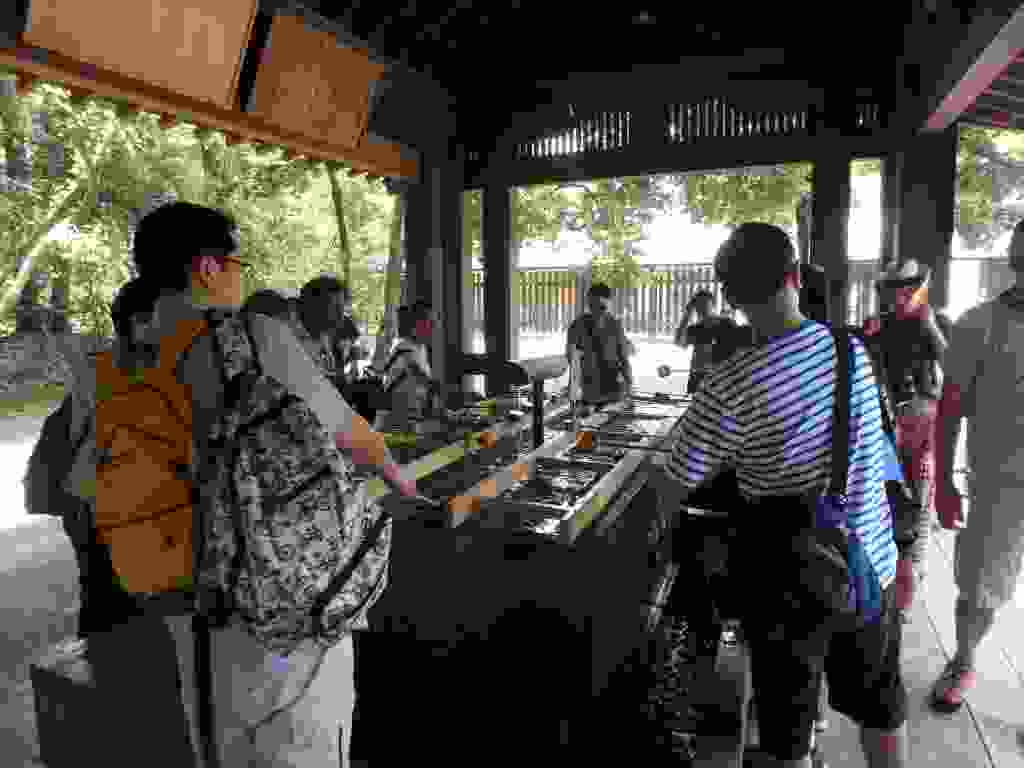
\includegraphics[width=\mywidth]{../wp-content/uploads/2015/07/P7205506-1024x768.jpg} } 
 \newline
 \newline
\centerline{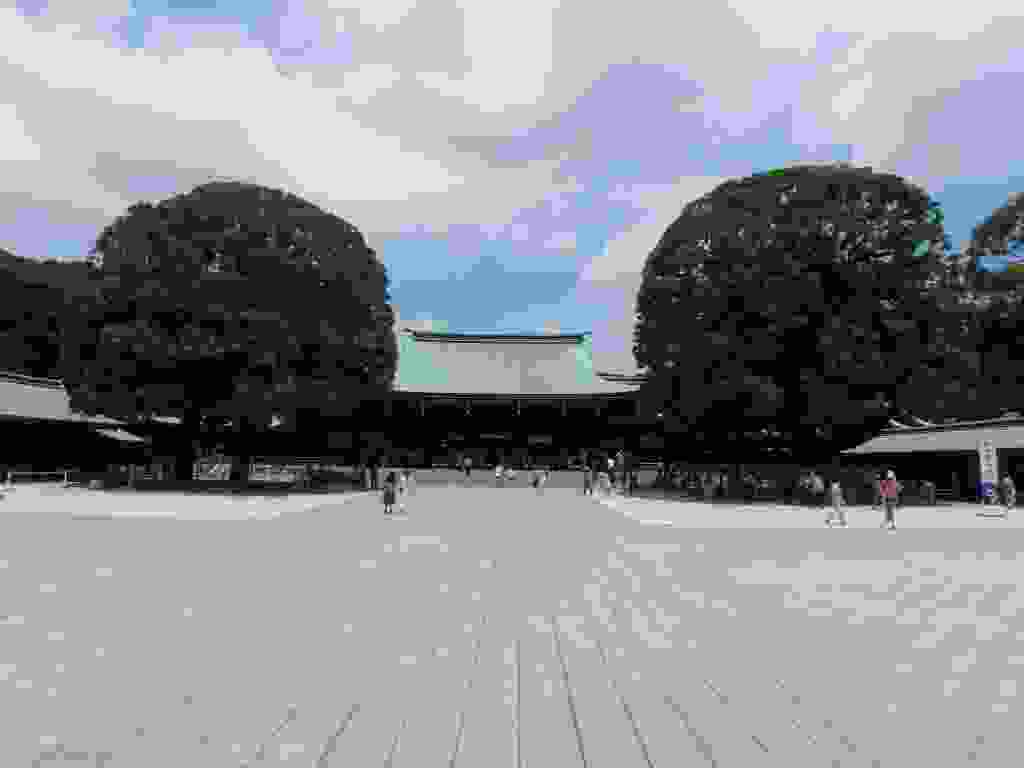
\includegraphics[width=\mywidth]{../wp-content/uploads/2015/07/P7205510-1024x768.jpg} } 
 \newline
 \newline
\centerline{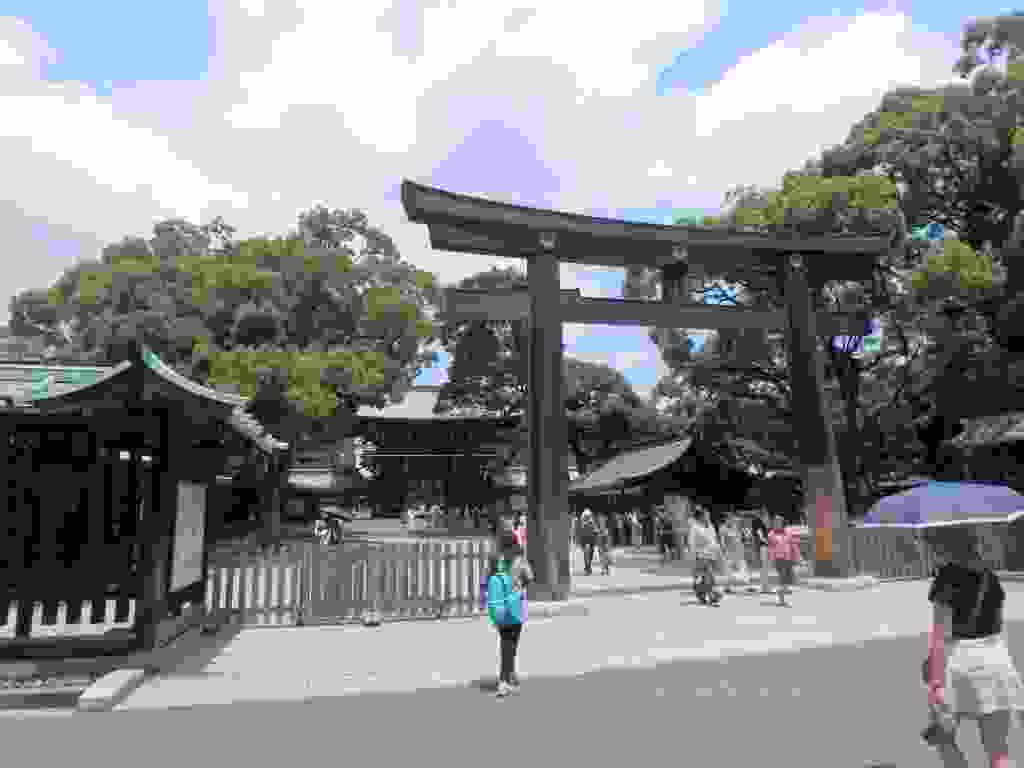
\includegraphics[width=\mywidth]{../wp-content/uploads/2015/07/P7205507-1024x768.jpg} } 
 \newline
 Akihabara et son «electric area», jeux vidéo, manga, maid bar… \newline
 \newline
\centerline{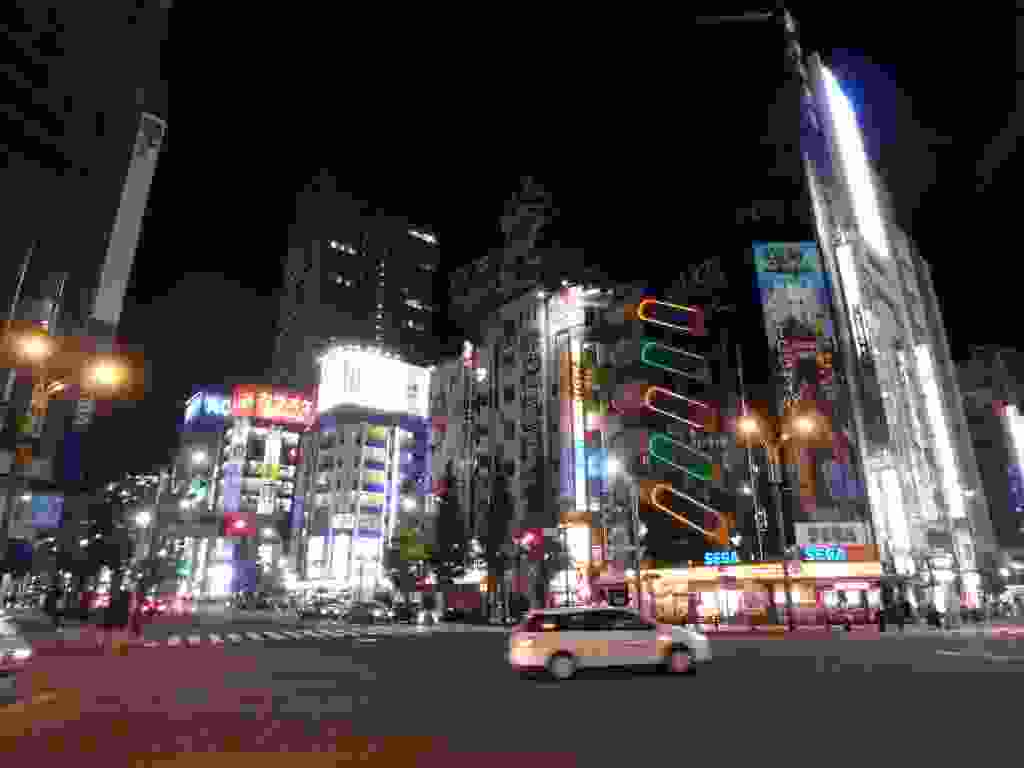
\includegraphics[width=\mywidth]{../wp-content/uploads/2015/07/P7225581-1024x768.jpg} } 
 \newline
 \newline
\centerline{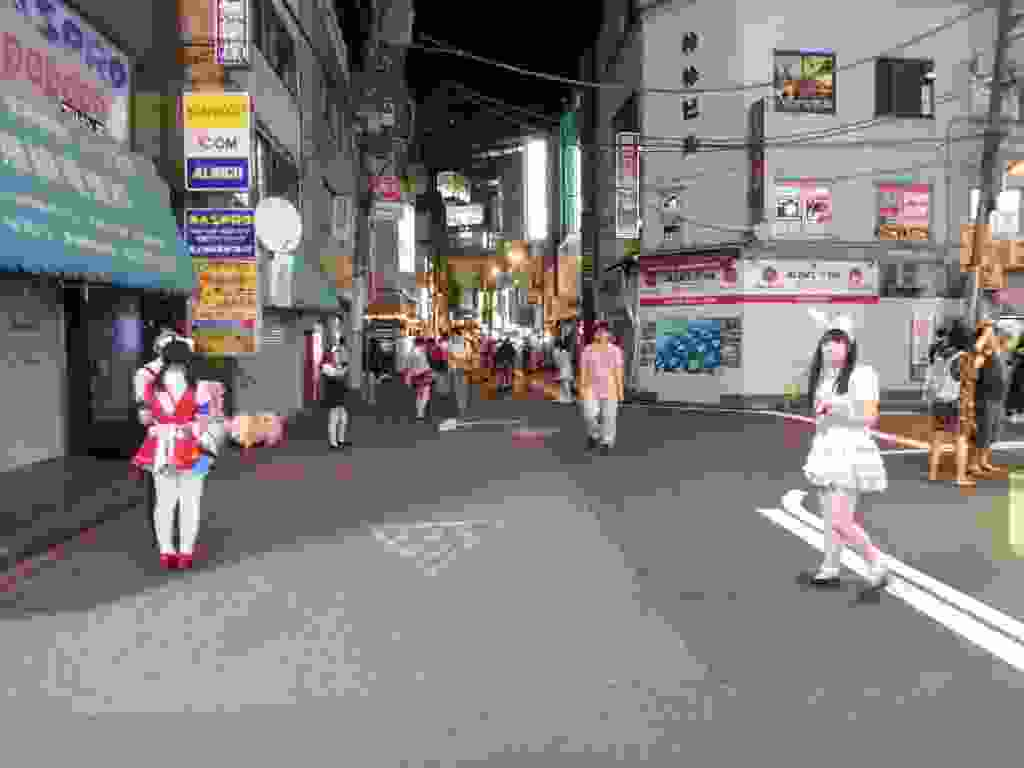
\includegraphics[width=\mywidth]{../wp-content/uploads/2015/07/P7225583-1024x768.jpg} } 
 \newline
 Dans le meme quartier le shrine Yushokan Yasukuni-jinja \newline
 \newline
\centerline{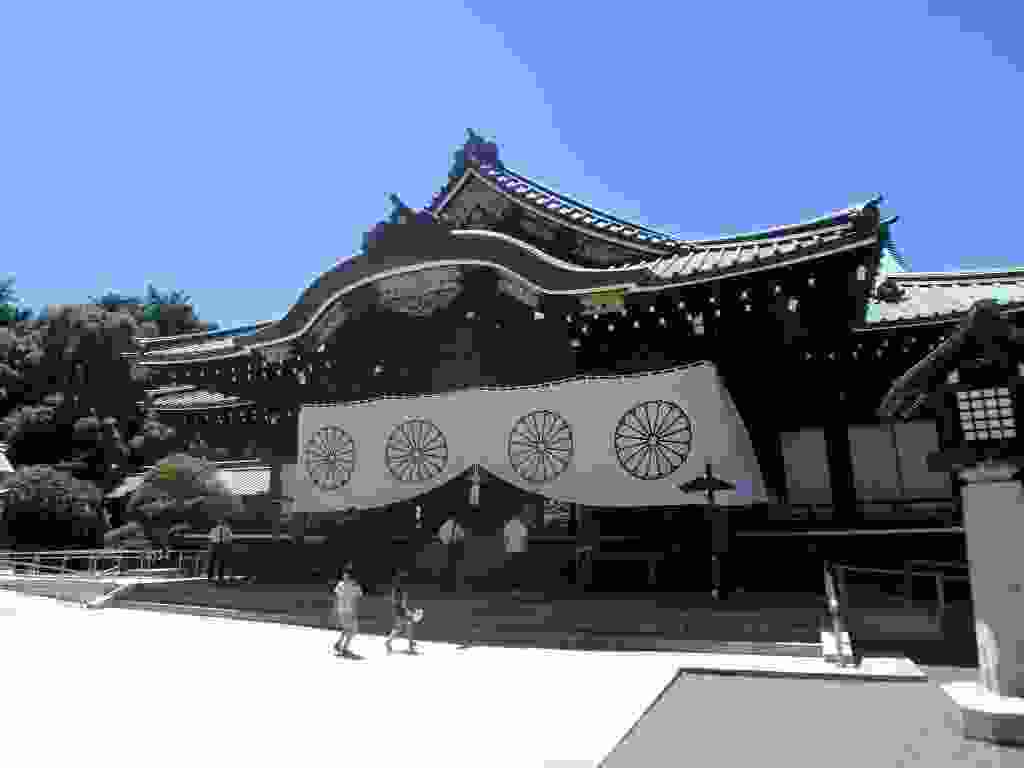
\includegraphics[width=\mywidth]{../wp-content/uploads/2015/07/P7225559-1024x768.jpg} } 
 \newline
 Le quartier Ueno et son grand parc qui contient de beaux temples et shrines. \newline
 \newline
\centerline{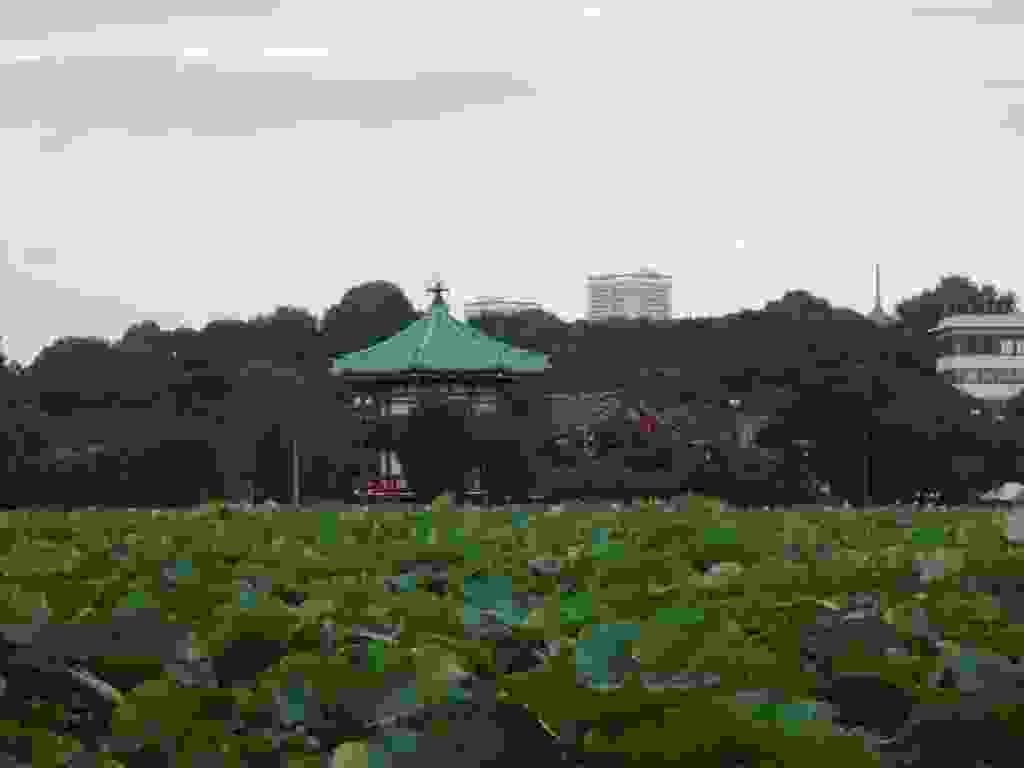
\includegraphics[width=\mywidth]{../wp-content/uploads/2015/07/P7195486-1024x768.jpg} } 
 \newline
 \newline
\centerline{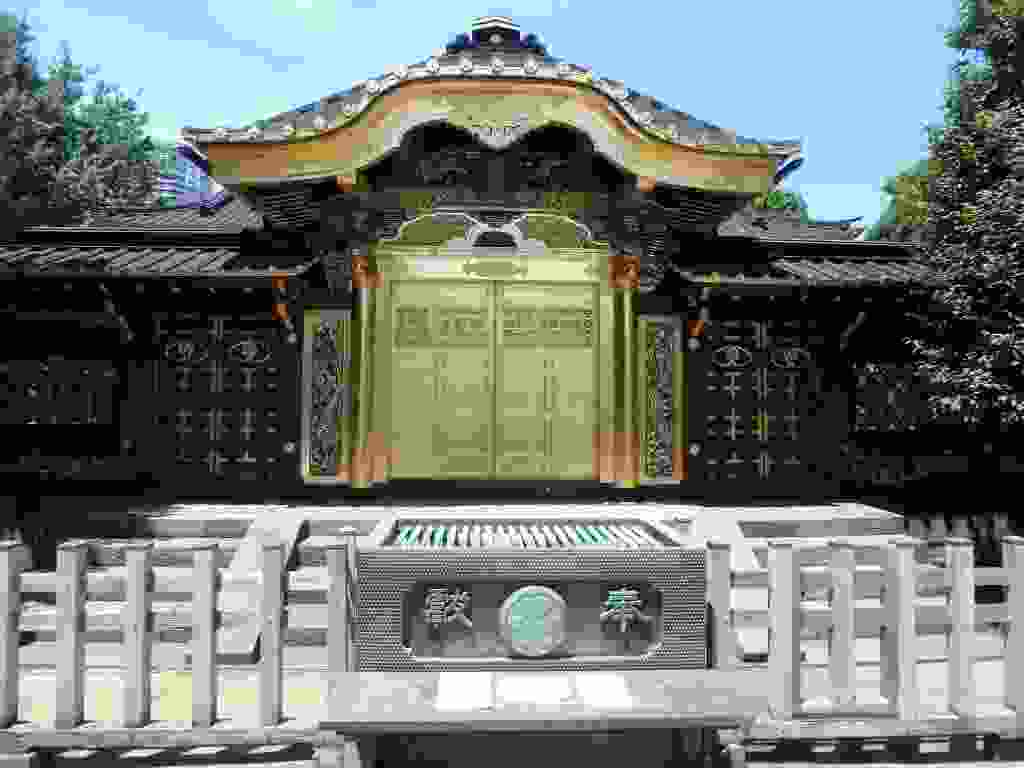
\includegraphics[width=\mywidth]{../wp-content/uploads/2015/07/P7195441-1024x768.jpg} } 
 \newline
 \newline
\centerline{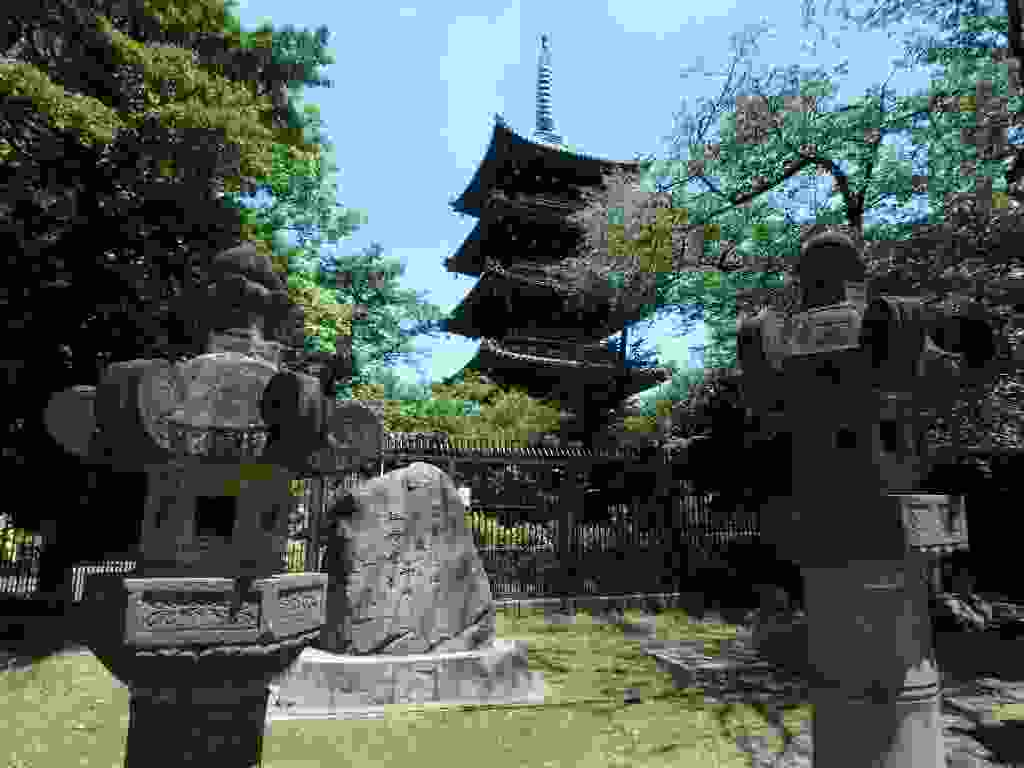
\includegraphics[width=\mywidth]{../wp-content/uploads/2015/07/P7195444-1024x768.jpg} } 
 \newline
 Le temple Kaneiji \newline
 \newline
\centerline{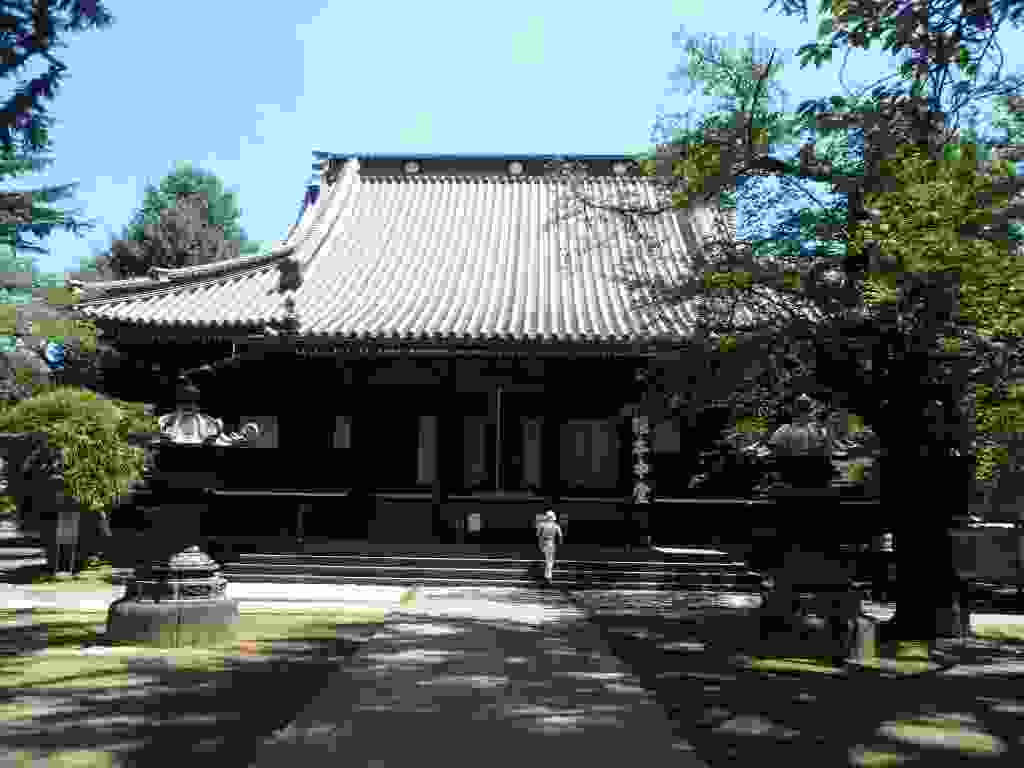
\includegraphics[width=\mywidth]{../wp-content/uploads/2015/07/P7195452-1024x768.jpg} } 
 \newline
 Shrine Yushima Tenmangu \newline
 \newline
\centerline{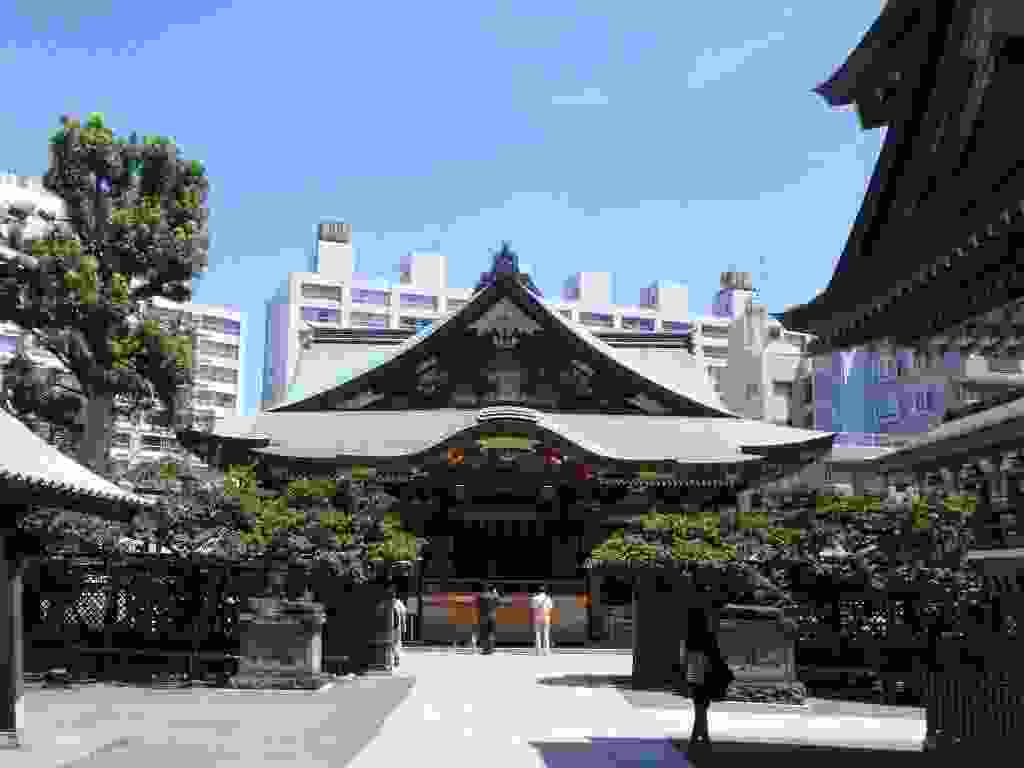
\includegraphics[width=\mywidth]{../wp-content/uploads/2015/07/P7195430-1024x768.jpg} } 
 \newline
 Un peu plus loin, le quartier Asakusa \newline
 La rue commerçante Nakamise, l'alignement de boutiques date de l'époque d'Edo (ancien nom de Tokyo). \newline
 \newline
\centerline{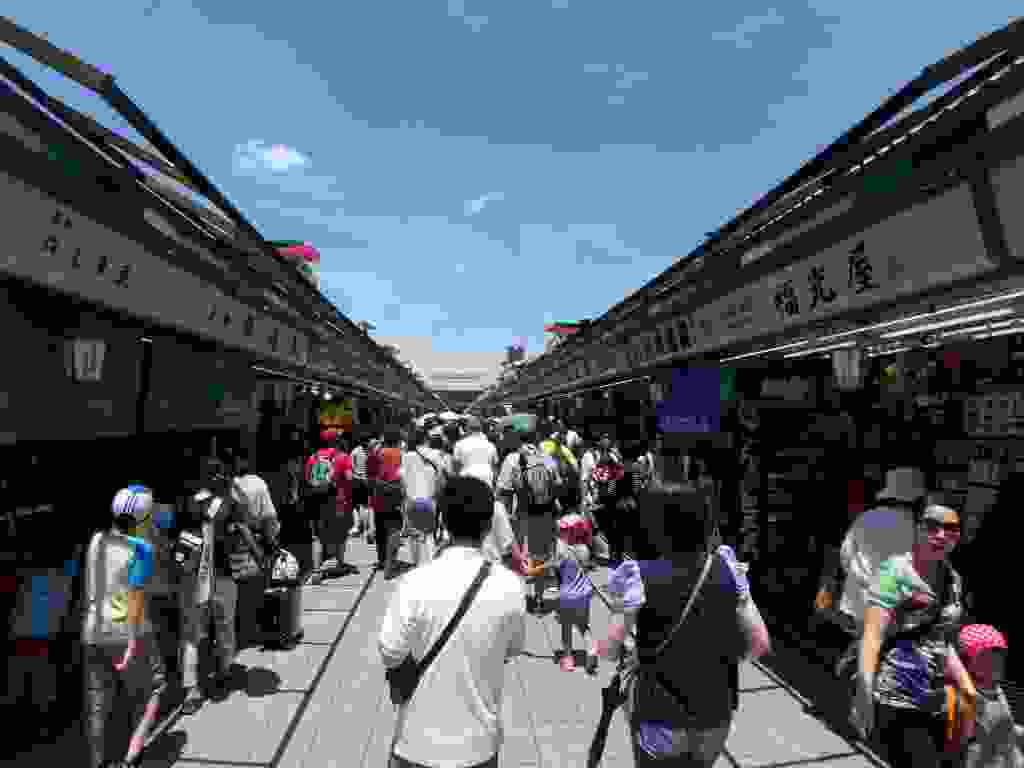
\includegraphics[width=\mywidth]{../wp-content/uploads/2015/07/P7195457-1024x768.jpg} } 
 \newline
 Le célèbre Temple Sensoji \newline
 \newline
\centerline{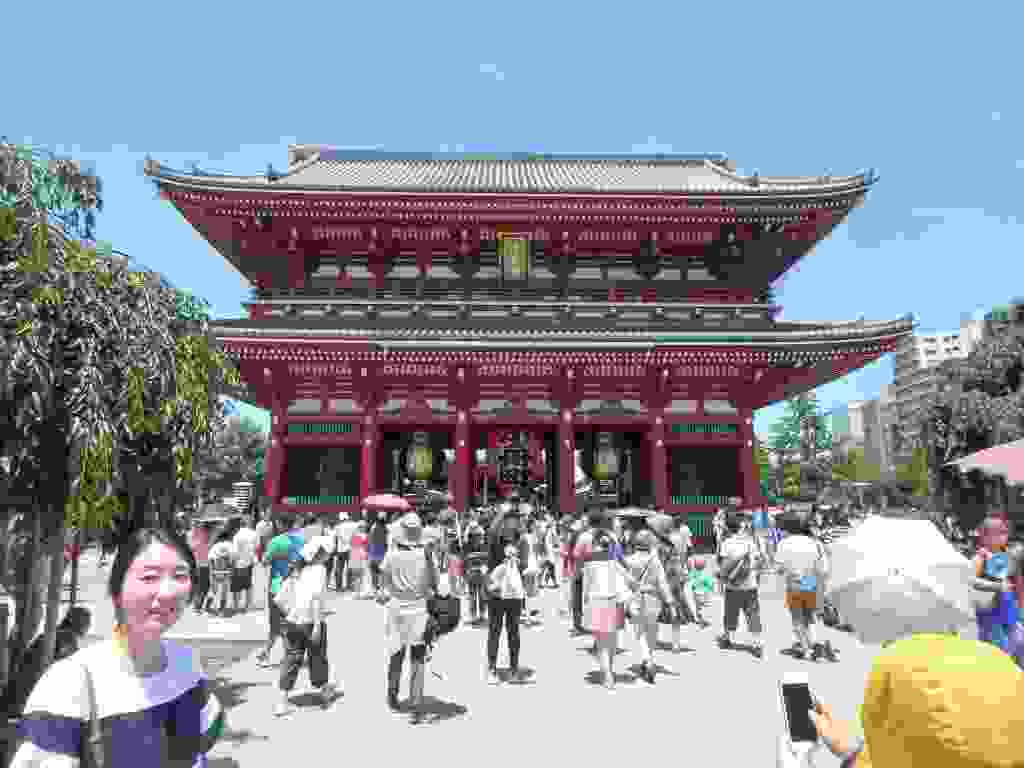
\includegraphics[width=\mywidth]{../wp-content/uploads/2015/07/P7195458-1024x768.jpg} } 
 \newline
 \newline
\centerline{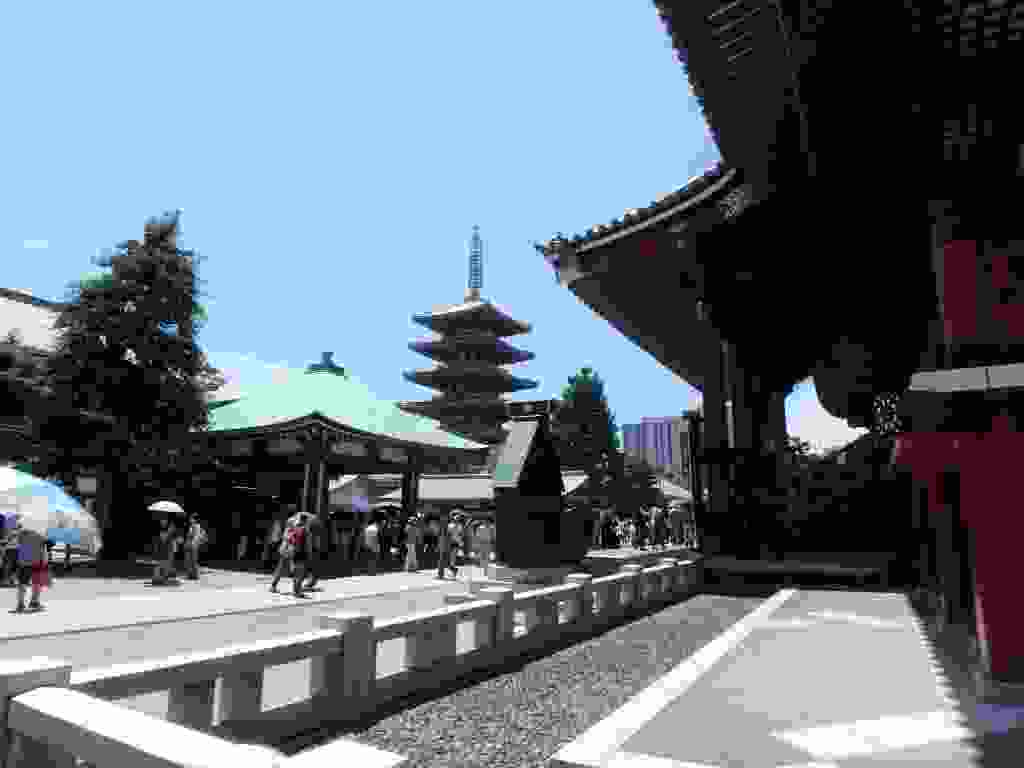
\includegraphics[width=\mywidth]{../wp-content/uploads/2015/07/P7195466-1024x768.jpg} } 
 \newline
 \newline
\centerline{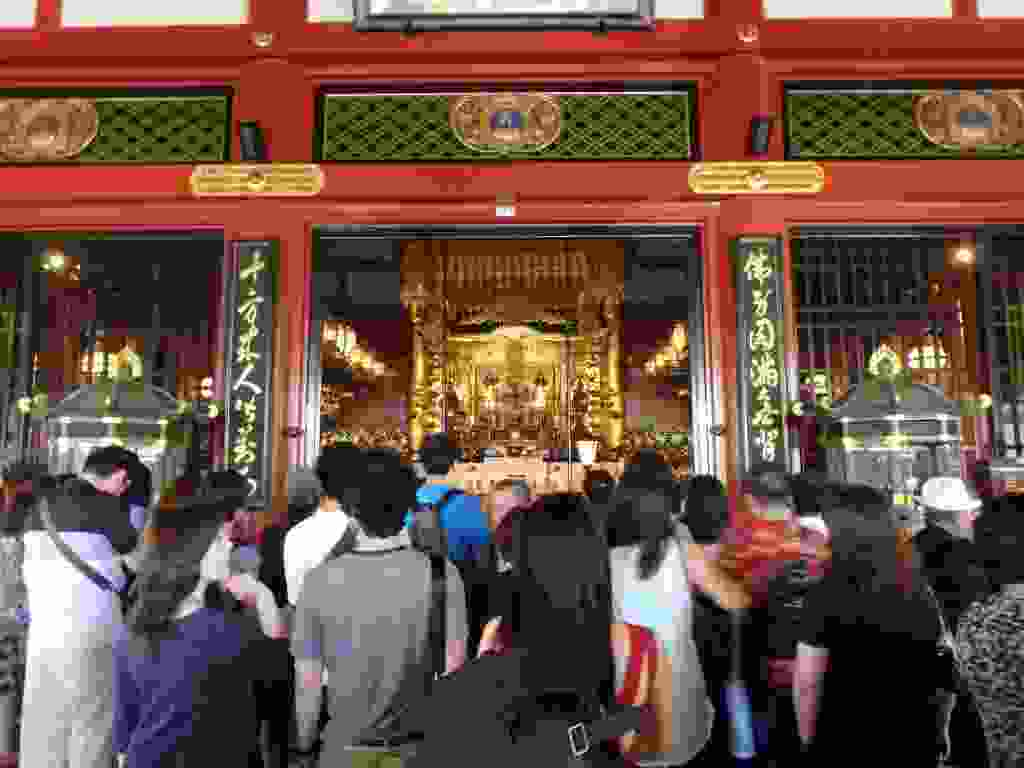
\includegraphics[width=\mywidth]{../wp-content/uploads/2015/07/P7195464-1024x768.jpg} } 
 \newline
 La tour Skytree \newline
 \newline
\centerline{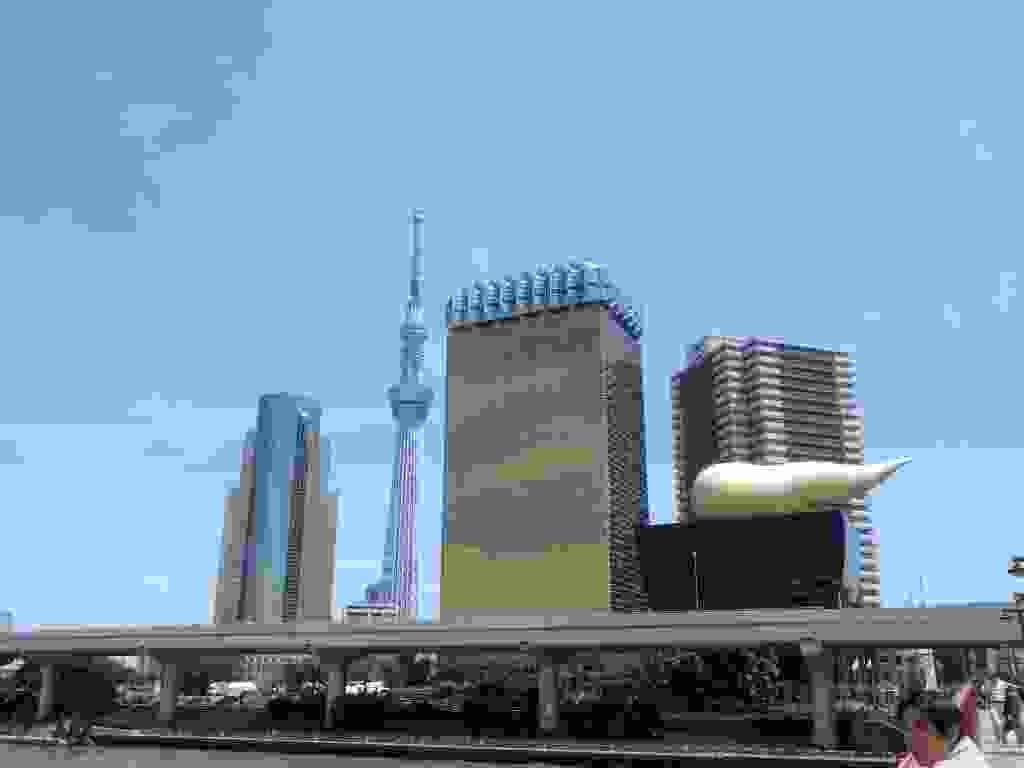
\includegraphics[width=\mywidth]{../wp-content/uploads/2015/07/P7195472-1024x768.jpg} } 
 \newline
 Je me suis déplacé la plupart du temps en vélo mais j'ai quand même testé une fois le métro, je m'attendais à ce qu'il soit plus bondé ! \newline
 \newline
\centerline{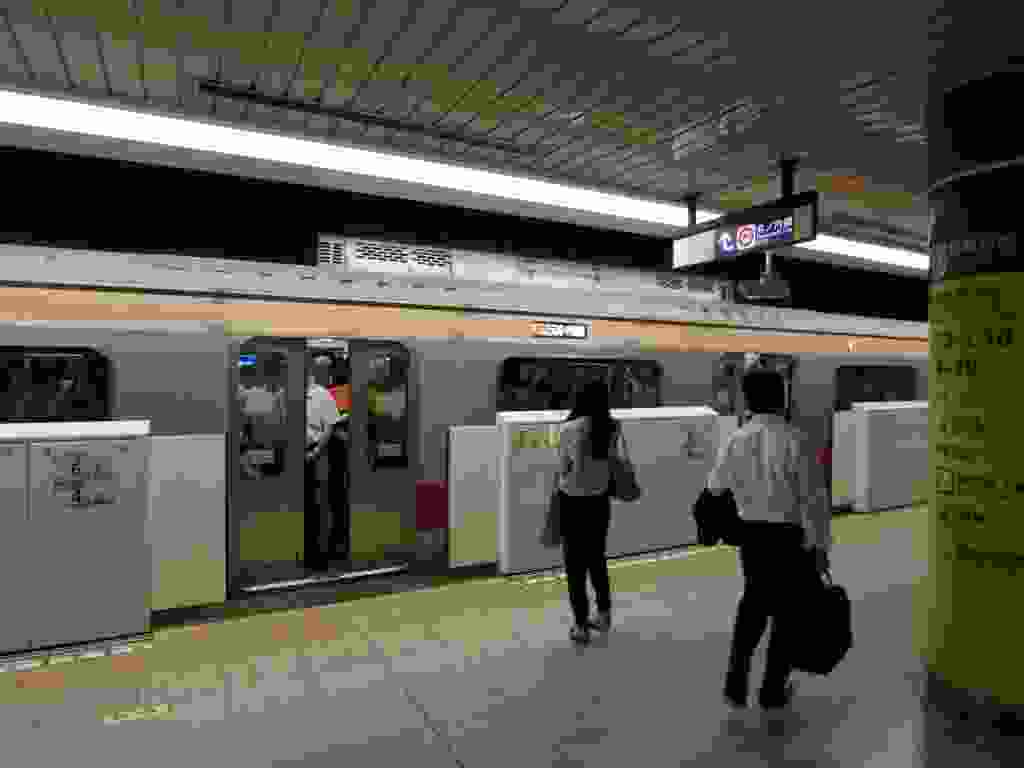
\includegraphics[width=\mywidth]{../wp-content/uploads/2015/07/P7215527-1024x768.jpg} } 
 \newline
 \newline
\centerline{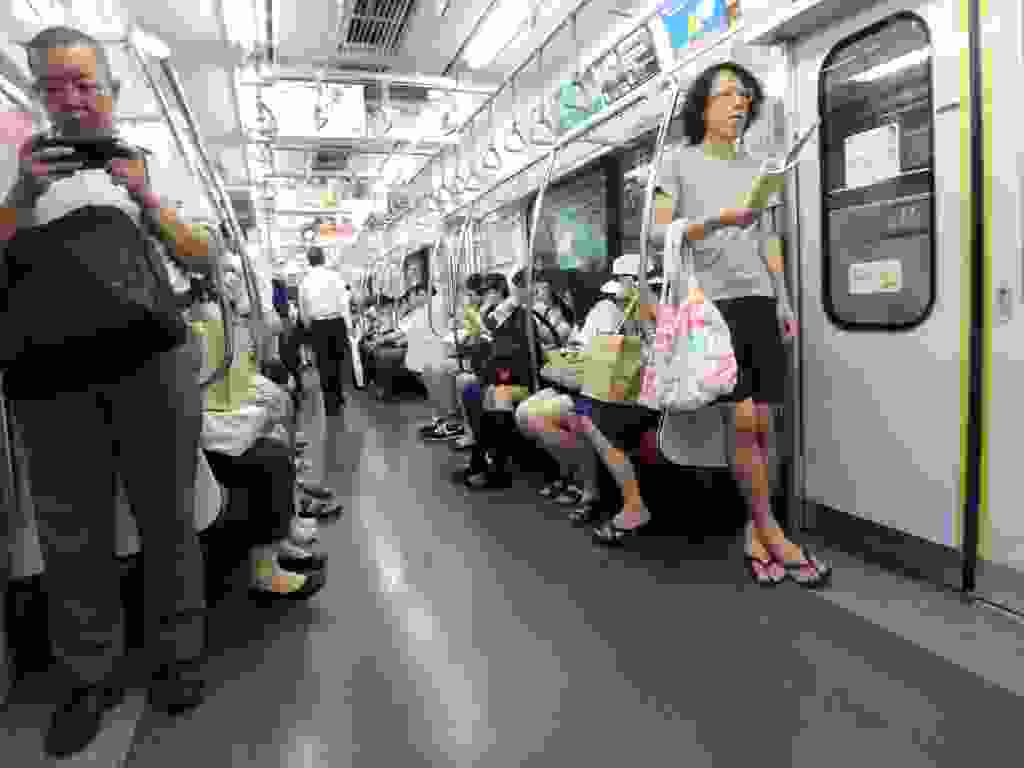
\includegraphics[width=\mywidth]{../wp-content/uploads/2015/07/P7215528-1024x768.jpg} } 
 \newline
 Je me suis arrêté une nuit dans le quartier Ikebukuro pour tester un hôtel capsule : tout le confort necessaire est la ! \newline
 \newline
\centerline{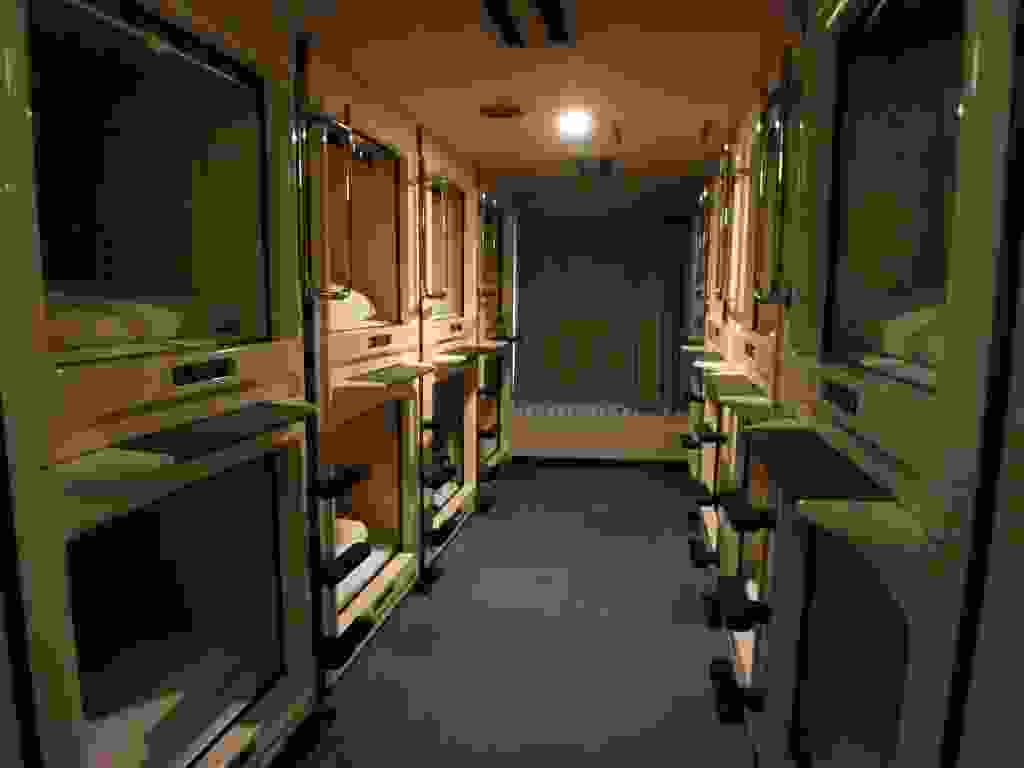
\includegraphics[width=\mywidth]{../wp-content/uploads/2015/07/P7205520-1024x768.jpg} } 
 \newline
 \newline
\centerline{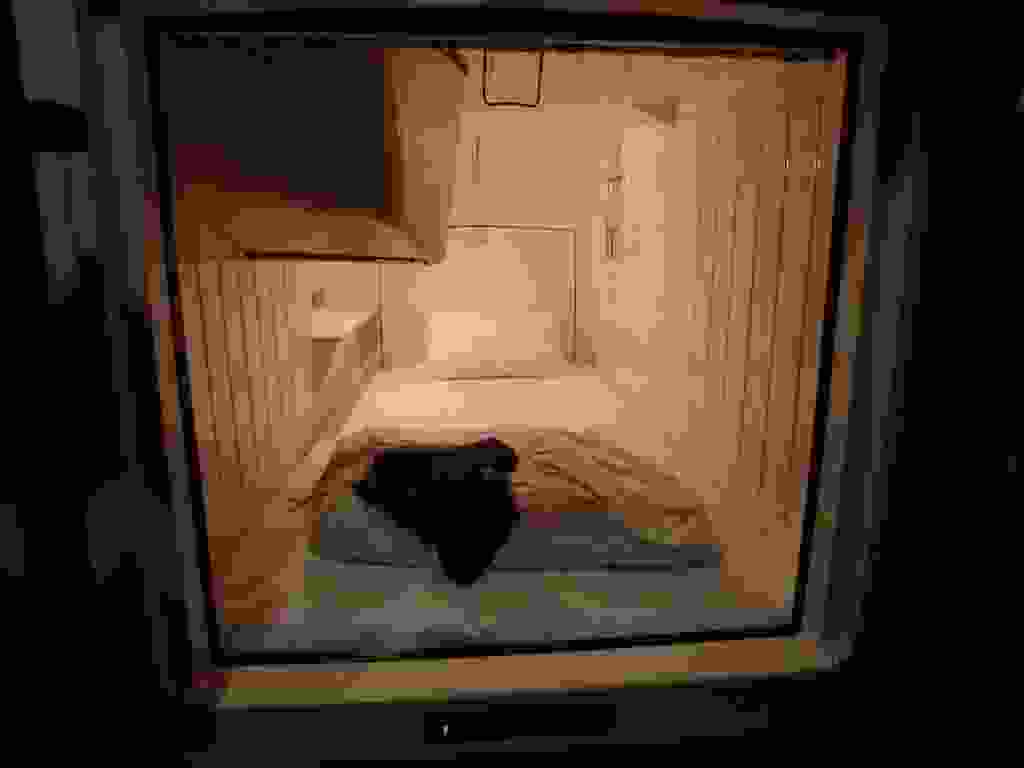
\includegraphics[width=\mywidth]{../wp-content/uploads/2015/07/P7205523-1024x768.jpg} } 
 \newline
 J'ai ensuite été accueilli par Yukiko et Carlos dans leur bel appartement de style japonais. Yukiko est guide pour des visites touristiques de Tokyo en vélo. \newline
 \newline
\centerline{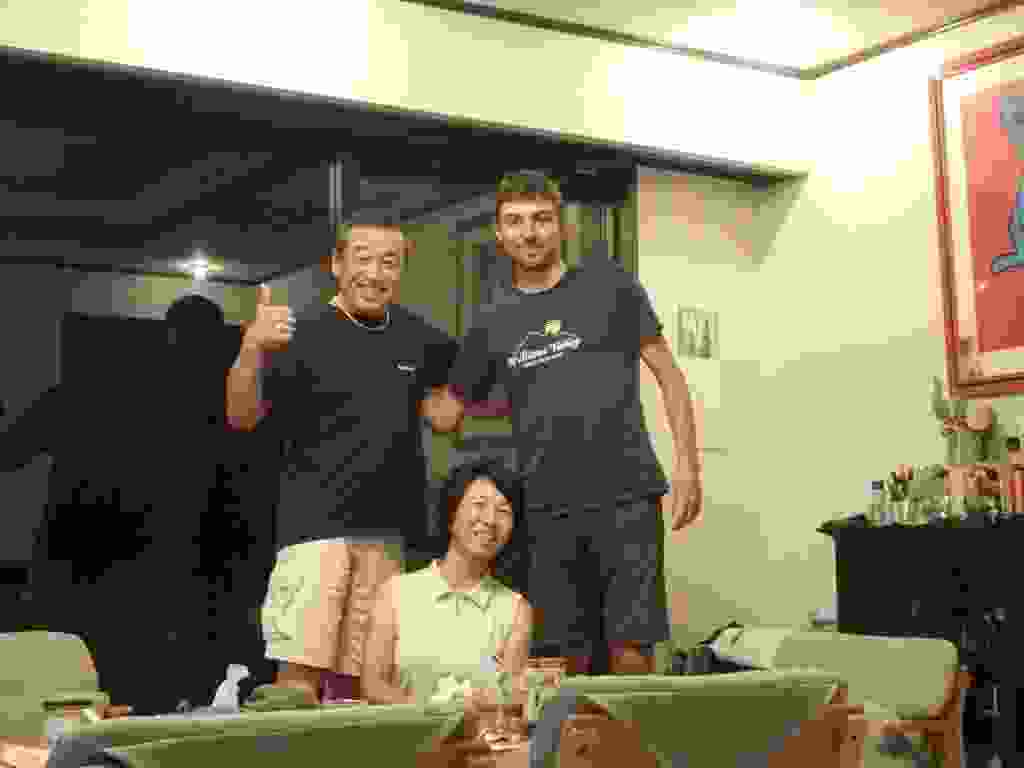
\includegraphics[width=\mywidth]{../wp-content/uploads/2015/07/P7235588-1024x768.jpg} } 
 \newline
 \newline
\centerline{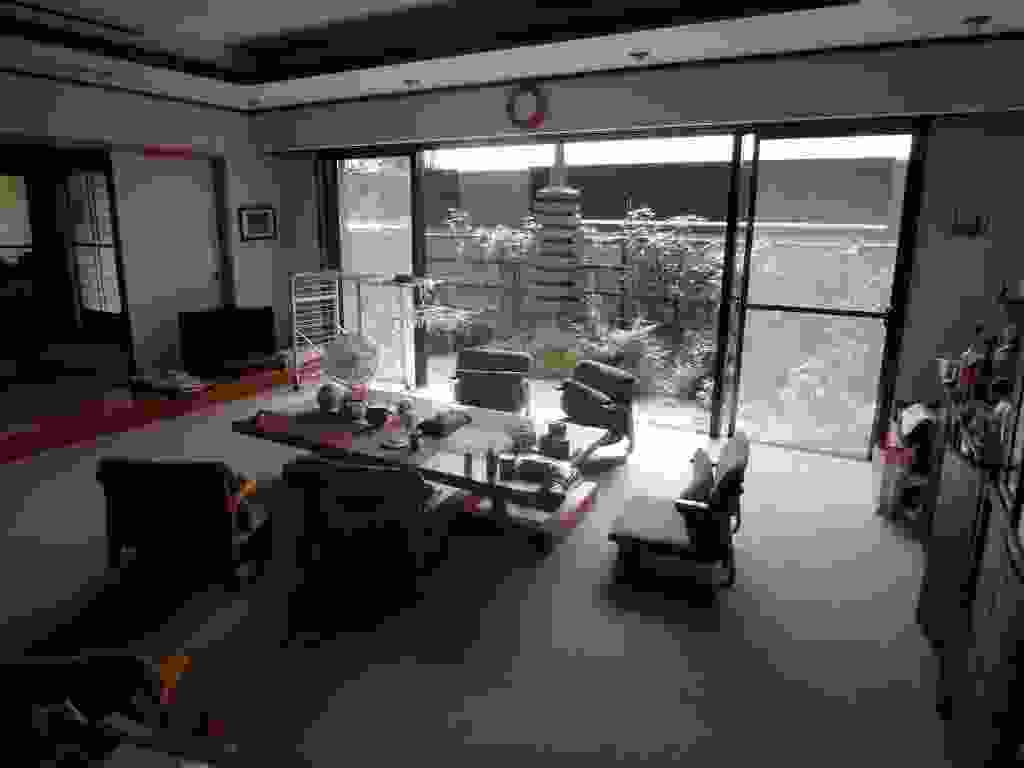
\includegraphics[width=\mywidth]{../wp-content/uploads/2015/07/P7225549-1024x768.jpg} } 
 \newline
 Ils habitent dans le quartier de Kagurazaka. Il y avait un festival avec un défilé, beaucoup de japonais portent un costume traditionnel. \newline
 \newline
\centerline{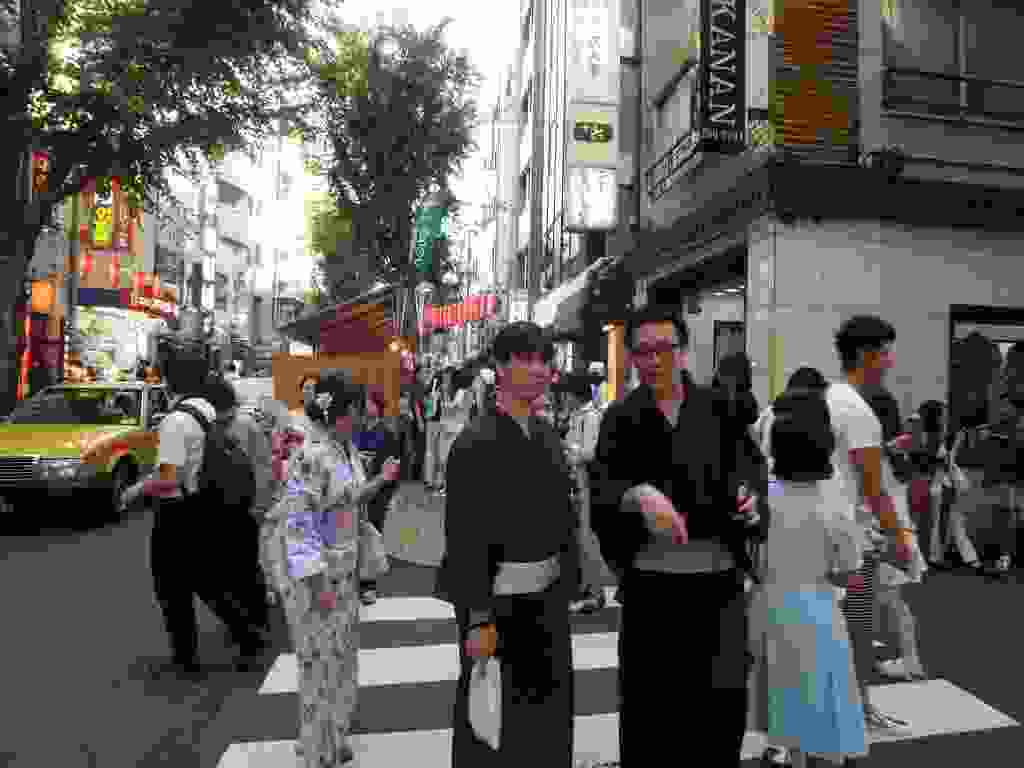
\includegraphics[width=\mywidth]{../wp-content/uploads/2015/07/P7235587-1024x768.jpg} } 
 \newline
 \newline
\centerline{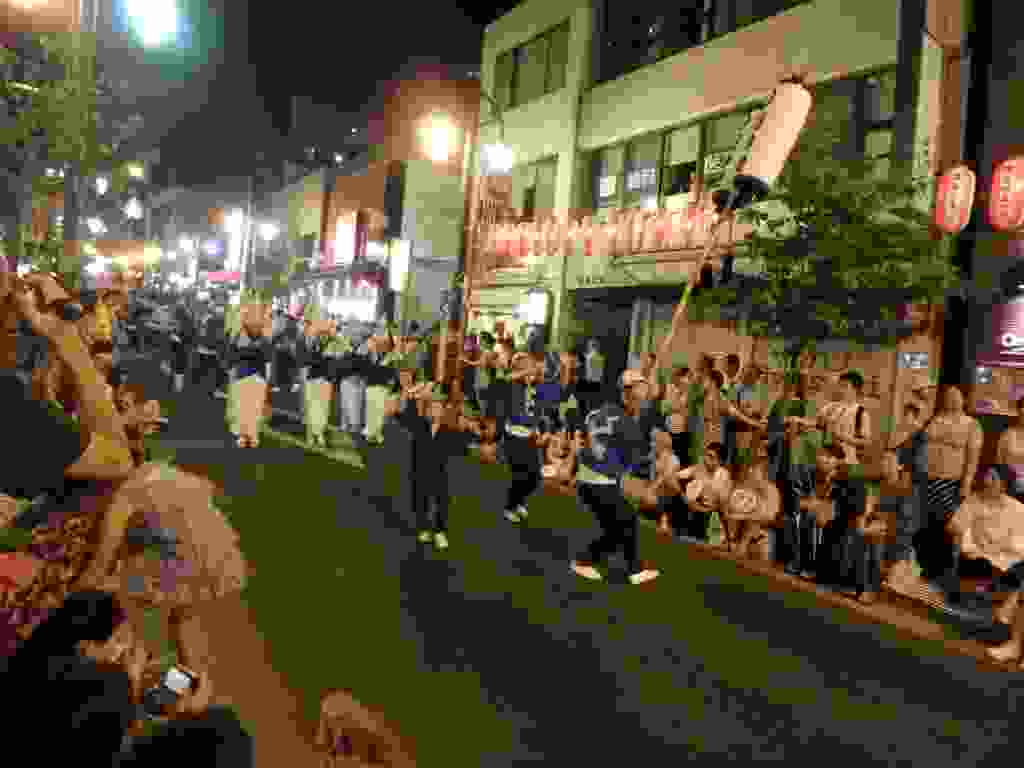
\includegraphics[width=\mywidth]{../wp-content/uploads/2015/07/P7245604-1024x768.jpg} } 
 \newline
 \newline
\centerline{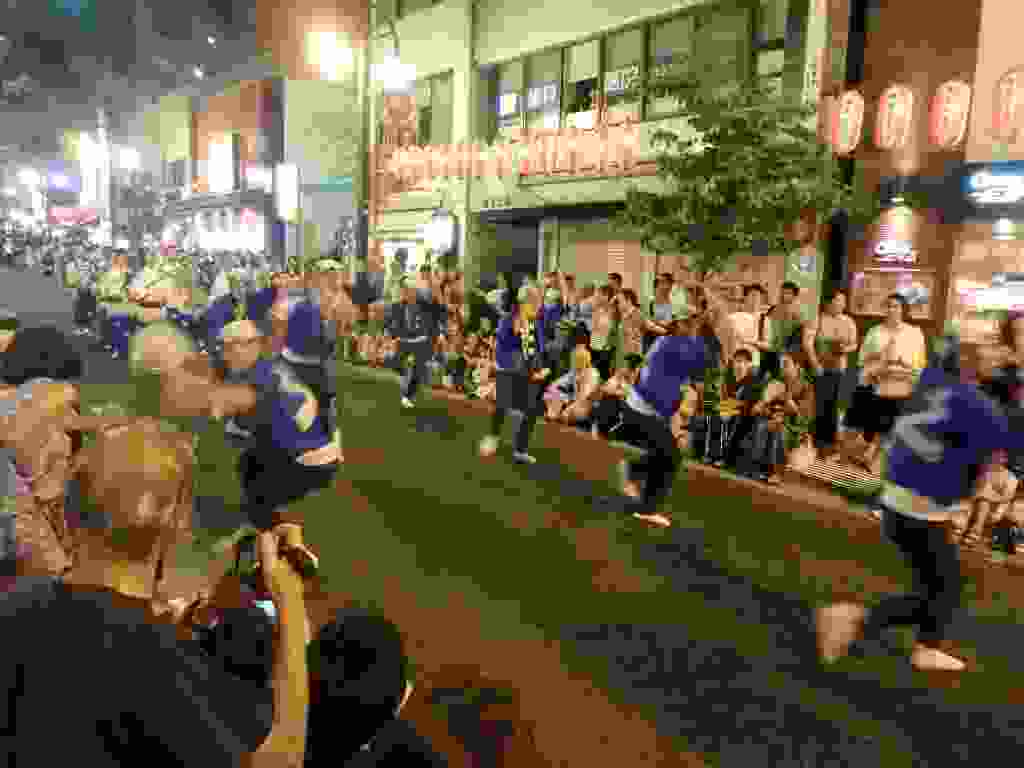
\includegraphics[width=\mywidth]{../wp-content/uploads/2015/07/P7245607-1024x768.jpg} } 
 \newline
 Repas dans un petit restaurant japonais, des spécialités originales et du saké : pas très fort et bon, ça ne ressemblait pas à ce que j'avais goûté en France. \newline
 \newline
\centerline{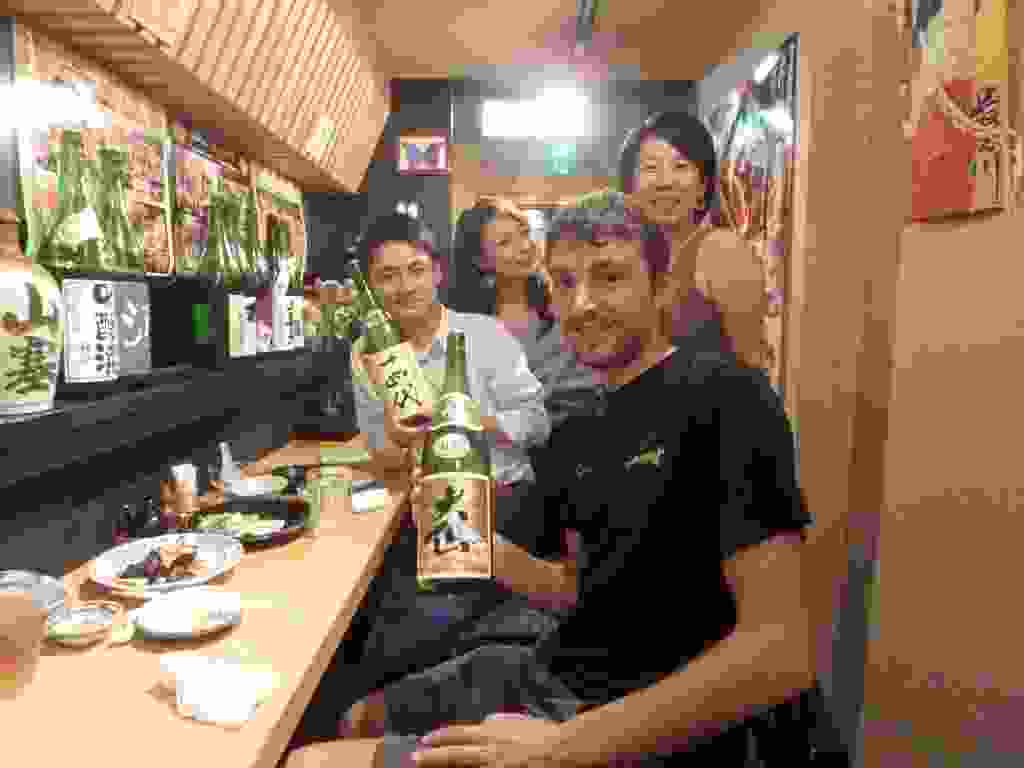
\includegraphics[width=\mywidth]{../wp-content/uploads/2015/07/P7245622-1024x768.jpg} } 
 \newline
 Quelques curiosités japonaises pour finir. \newline
 Toilettes high-tech \newline
 \newline
\centerline{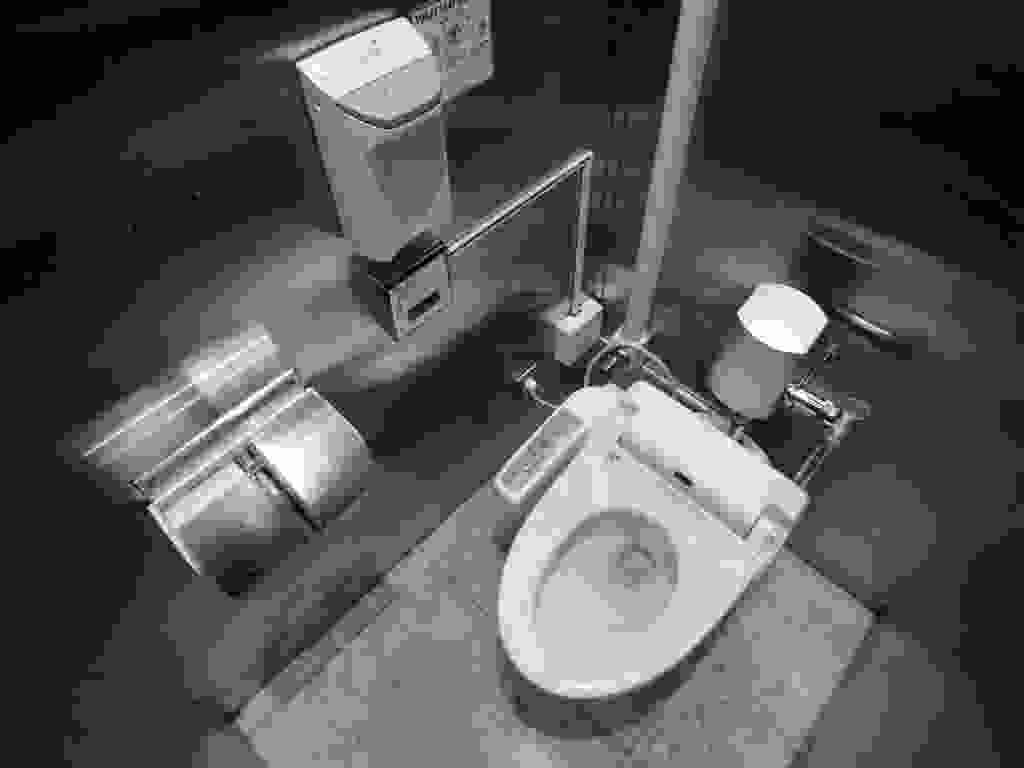
\includegraphics[width=\mywidth]{../wp-content/uploads/2015/07/OI000004-1024x768.jpg} } 
 \newline
 Les «convenience stores» quasiment à tous les coins de rues, ils font supermarchés, plats préparés, café, distributeur d'argent, journaux, tabac, toilettes… \newline
 \newline
\centerline{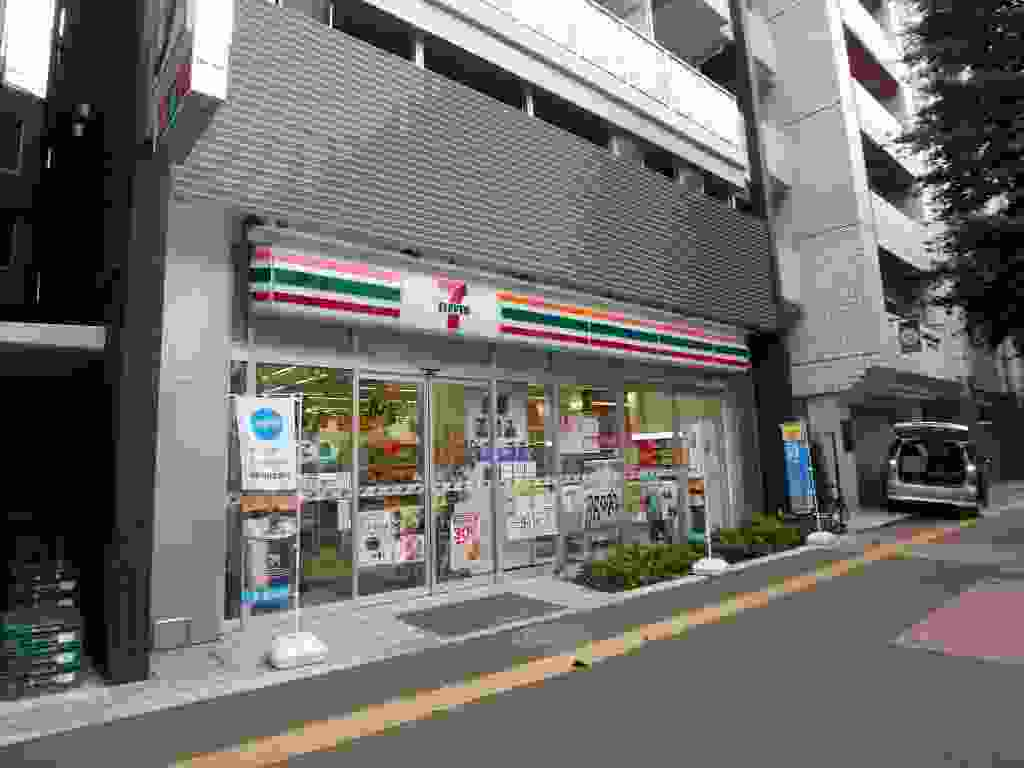
\includegraphics[width=\mywidth]{../wp-content/uploads/2015/07/P7195488-1024x768.jpg} } 
 \newline
 Vitrine de restaurant avec des reproduction des plats, pratique pour choisir. \newline
 \newline
\centerline{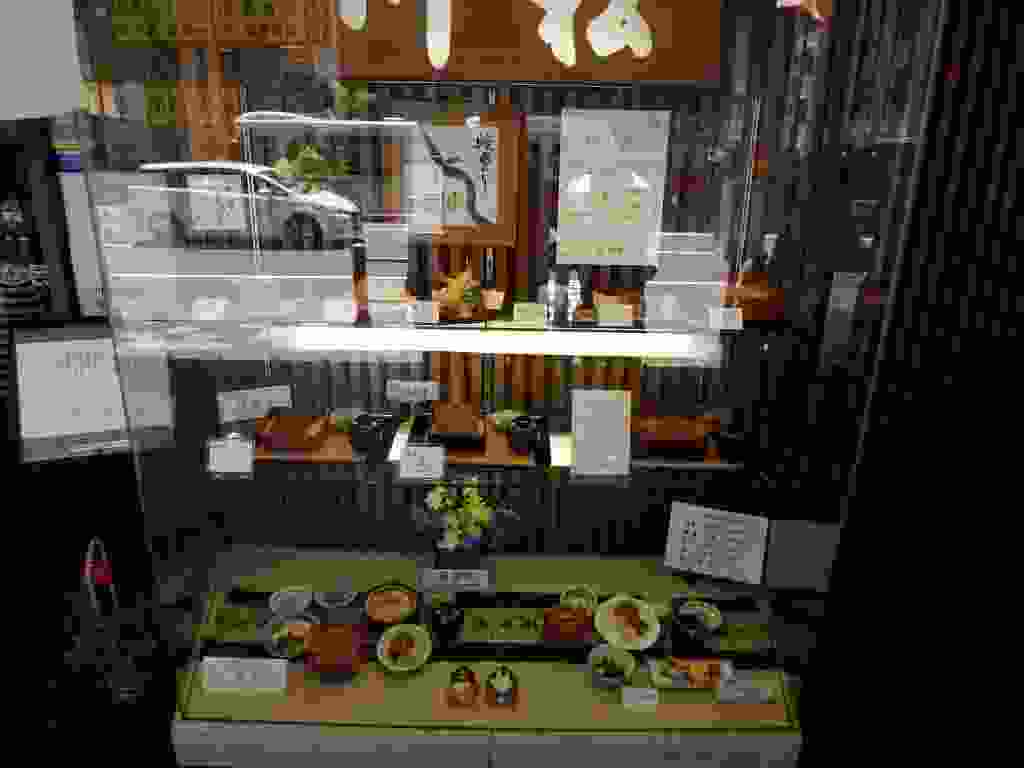
\includegraphics[width=\mywidth]{../wp-content/uploads/2015/07/P7195471-1024x768.jpg} } 
 \newline

\newpage
 
